%
% METU Institute of Natural and Applied Sciences Thesis example 
%
% Edited and Commented by Utku Erdoğdu 2013
% Modified for IAM - Institute of Applied Mathematics
% Graduate School of Applied Mathematics
% Edited and Commented by Omur Ugur 2017-2018
%
% Please read the explanations so that you can customize the document		
%
% Files needed by this document:
% metu.cls 
% metu11.def (if you will use 11pt fonts) 
% metu12.def (if you will use 12pt fonts)
% metu10.def (if you will use 10pt fonts)
%
% Possible Options Here:
%
% oneandhalf, double, single : Line spacing used in the thesis. 
% Default and institute preference is
% single.
%
% 10pt, 11pt, 12pt : Font size Default is 10pt, which is institue choice. 
% 
% pntr, pntc, pnbt : Page number position. 
% Options are top center, top right or bottom. 
% Default and institute preference is page numbers at bottom. 
% When page numbers are at the top bottom margins are skewed.
% 
% chaproman, chaparabic: Chapter numbering format. 
% Options are roman numbers and arabic numbers.
% Default is roman, institute prefers arabic
%
% oneside, twoside : Printing style. Default is twoside. 
% In this style chapters and (almost all) preliminary pages begin from 
% odd numbered pages.
%
% tr, eng : Document language. This is useful if you want to translate 
% your thesis into Turkish. 
% Then you give the option tr and use \ifturkish. . .\else. . .\fi  
% whenever you want 
% to do something only for Turkish or only for English. Default is eng. 
% IMPORTANT!! : For official institute documents you should not use this option. 
% The Turkish format is only supplied for custom translations.
%
% ceng,aee,arme.. : You can use the abbreviated form of your department here 
% and there is no further need to define the department name below. 
% If your department name is not among the below list of defined
% departments, you should use \department and \turkishdepartment macros 
% to define the name of your department.
%
% Defined Departments and Abbreviations:
% (may not work after modification for IAM)
% --------------------------------------
% Computer Engineering : ceng
% Aerospace Engineering : aee
% Archaeometry : arme
% Architecture : arch
% Biochemistry : bch
% Biology : biol
% Biomedical Engineering : bme
% Biotechnology : btec
% Building Science : bs
% Cement Engineering : ceme
% Chemical Engineering : che
% Chemistry : chem
% City and Regional Planning : crp
% City Planning : cp
% Civil Engineering : ce
% Computational Design and Fabrication Technologies in Architecture : arcd
% Computer Education and Instructional Technology : cte
% Design Research for Interaction : iddi
% Earthquake Studies : eqs
% Earth System Science : ess
% Electrical and Electronics Engineering : ee
% Engineering Management : em
% Engineering Sciences : es
% Environmental Engineering : enve
% Food Engineering : fde
% Geodetics - Geographical Information Technologies : ggit
% Geological Engineering : geoe
% Hydrosystems Engineering : he
% Industrial Design : id
% Industrial Engineering : ie
% Mathematics : math
% Mechanical Engineering : mech
% Metallurgical and Materials Engineering : mete
% Micro and Nanotechnology : mnt
% Mining Engineering : mine
% Operational Research : or
% Petroleum and Natural Gas Engineering : pete
% Physics : phys
% Polymer Science and Technology : pst
% Regional Planning : rp
% Restoration : rest
% Secondary Science and Mathematics Education : ssme
% Software Engineering : se
% Statistics : stat
% Structural Mechanics : st
% 
% phd, ms : Degree Received. Ph.D. or M.S. Default is M.S.
%
%
% Defined for use of IAM:
% acsc, cryp, fm, sc
%
% End of Options


% Use one of the following \documentclass with options of metu_iam.cls
\documentclass[chaparabic,sc,ms,12pt,oneandhalf]{metu_iam} 
%\documentclass[chaparabic,fm,ms,11pt,oneandhalf]{metu_iam} % preferred by IAM
%\documentclass[chaparabic,acsc,ms,10pt,single]{metu_iam} % preferred by the FBE
%\documentclass[chaparabic,cryp,phd,12pt,double]{metu_iam}

% You can delete next line If your thesis does not have an appendix
\usepackage{appendix}

%
% Personal Information 
% ----------------------------
%
% Please check this part and fill in information about your thesis
%
% Name and Surname
% be careful with the uppercase letters and Turkish characters
% following name should work for both UPPERCASE and LOWERCASE names
\author{UĞURCAN ÖZALP}
% Thesis Title English and Turkish
\title{Bipedal Robot Walking by Reinforcement Learning in Partially Observed Environment}
\turkishtitle{Pekiştirmeli Öğrenme Yöntemleriyle Kısmi Gözlenebilir Ortamda Çift Bacaklı Robotun Yürütülmesi}
% Department : English and Turkish
%
% Some of the departments are pre-defined, you need not redeclare them. 
% You can use them by just giving an option to \documentclass. 
% See documentation for options above. If you will define your 
% department here do not use ``Department'' or ``Bölümü'' words.
%\department{Computer Engineering}
%\turkishdepartment{Bilgisayar Mühendisliği}
%
% Date : You should indicate the month of your thesis defence in English.
% Default is this month
%
\date{July 2021} % do NOT use comma
%
% Approval Page Details
% --------------------------
% For each command you can give the title as optional parameter enclosed in [ ]
% This also handles the Turkish titles if you're planning 
% to produce Turkish version of the document. 
% If you'll hard code the title, you need 
% to use turkish version of each command after the command itself
% 
% prof : Prof. Dr.
% assocprof : Assoc. Prof. Dr.
% assistprof : Assist. Prof. Dr.
% dr : Dr.
%
% Director of Institute
\director[prof]{A. Sevtap Selçuk-Kestel}
% Head of Department
\headofdept[prof]{Hamdullah Yücel}
%
% Supervisor : English and Turkish
\supervisor[prof]{Ömür Uğur}
%\cosupervisor[assistprof]{Noname NoSurname} % suppress/comment if you don't have cosupervisor
% \turkishsupervisor{  } %if you will hard-code the academic title
%
% Affiliation of Supervisor in English and possibly in Turkish
\departmentofsupervisor{Scientific Computing, METU}
% \turkishcosupervisor{Prof. Dr. Reda Alhajj} %if you will hard-code the academic title
% Affiliation of Co-Supervisor
% You can just delete/comment the next line if you don't have a co-supervisor
%\departmentofcosupervisor{Computer Engineering Dept., Bilkent Uni.}
%
% Committee Members
% In general members are sorted according to their academic titles; however
% new modifications indicate
%
% The Chair (1)
% Supervisor (2)
% Co-supervisor, if any (3)
% Academic Titles (4,5) or (3-5)
% 
% IMPORTANT:  All affiliatons should fit in a single line
% If affiliation line is broken into two lines you should shorten the affiliation by using 
% abbrevations or any other means
%
\committeememberi[assocprof]{Ümit Aksoy}
\affiliationi{Mathematics, Atılım University}
% Second committee member is always your supervisor
\committeememberii[prof]{Ömür Uğur}
\affiliationii{Scientific Computing, METU}
% If you are an M.Sc. student and your Co-Supervisor is in your 
% examination committee, then third committee member is always your co-supervisor
%
% IMPORTANT: If you are Ph.D. student your co-supervisor cannot be in your 
% examination committee.
\committeememberiii[assistprof]{Önder Türk}
\affiliationiii{Scientific Computing, METU}

% Fourth committee member
% If you have only three (3) Committee Members;
% this can ONLY be if this is a M.Sc thesis
% then uncomment \committeeivfalse so that
% 4th and 5th members do NOT count at all:
%\committeeivfalse
% Otherwise, you need to fill in the 4th and the 5th members
\committeememberiv[assocprof]{Ceylan Yozgatlıgil}
\affiliationiv{Statistics, METU}
% Fifth committee member is a MUST if Fourth committee member is
\committeememberv[prof]{Ayhan Aydın}
\affiliationv{Mathematics, Atılım University}
%
% Keywords : English & Turkish, Comma seperated
\keywords{deep reinforcement learning, partial observability, robot control, actor-critic methods, long short term memory, transformer}
\anahtarklm{pekiştirmeli derin öğrenme, kısmi gözlemlenebilirlik, robot kontrolü, aktör-eleştirmen metodları, uzun kısa süreli bellek, transformatör}

%
% Abstract in English
%
\abstract{
% either write abstract here or simply input
Deep Reinforcement Learning methods on mechanical control are successful on many environments and used instead of traditional optimal and adaptive control methods on some complex cases. However, Deep Reinforcement Learning algorithms do still have challenges. One is control on partially observable environments. When an agent is not informed well about the environment, it must recover information from past observations. In this thesis, walking of Bipedal Walker (OpenAI GYM) environment is studied by continious actor-critic reinforcement learning algorithm Twin Delayed Deep Determinstic Policy Gradient. Environment is partially observable because walker is not able to see behind. Several neural architectures are implemented. First one is Residual Feed Forward Neural Network under the observable environment assumption, while second and third ones are Long Short Term Memory and Transformer using observation history as input to recover hidden state since environment is assumed to be partially observable.



 % filename: abstract.tex
}
%
% Turkish Abstract
%
\oz{
% either write öz here or simply input
Mekanik kontrol üzerine Derin Pekiştirmeli Öğrenme yöntemleri birçok ortamda başarılıdır ve bazı karmaşık durumlarda geleneksel optimal ve uyarlanabilir kontrol yöntemleri yerine kullanılır. Ancak, Derin Pekiştirmeli Öğrenme algoritmalarının hala zorlukları vardır. Bunlardan biri kısmen gözlemlenebilir ortamlarda kontroldür. Bir özne ortam hakkında yeterince bilgilendirilmediğinde, geçmiş gözlemleri anlık gözlemlere ek olarak kullanmalıdır. Bu tezde, Bipedal Walker (Çift bacaklı yürüyen robot, OpenAI GYM) ortamının yürüyüşü, sürekli aktör-eleştirmen pekiştirmeli öğrenme algoritması İkiz Gecikmeli Derin Belirleyici Poliçe Gradyanı ile incelenmiştir. Robot arkasını göremediği için çevre kısmen gözlemlenebilirdir. Çalışmada birkaç sinir mimarisi uygulanmıştır. Birincisi, gözlemlenebilir ortam varsayımı altında artık bağlantıya sahip ileri beslemeli sinir ağı iken, ikinci ve üçüncü olanlar, ortamın kısmen gözlemlenebilir olduğu varsayıldığından girdi olarak gözlem geçmişini kullanan Uzun Kısa Süreli Bellek (LSTM) ve Dönüştürücüdür (Transformer). % filename: oz.tex
} 
%
% Dedication 
\dedication{\textit{ For anyone who is curious to read. % better to write here as it is short enough
}}
%
%
% Acknowledgements   
\acknowledgments{
% either write acknowledgments here or simply input
I would like to thank my thesis supervisor Prof. Dr. Ömur U\u{g}ur whose insightful comments and suggestions were of inestimable value for my study. His willingness to give his time and share his expertise has paved the way for me. \\

Special thanks also go to my friend Mehmet Gökçay Kabataş whose opinions and information have helped me very much throughout the production of this study. \\

I would also like to express my gratitude to my family for their moral support and warm encouragements. Especially, I would like to show my greatest appreciation to Serpil Sökmen, who provides me to come these days. \\

Lastly, I would like to thank my partner Dilara Bayram for supporting me in long study days. \\
 % filename: acknowledgments.tex
}
%
% End of Personal and Introductory Information
%%%%%%%%%%%%%%%%%%%%%%%%%%%%%%%%%5

%%% !!! These are most probably you need for effective use of metu_iam.cls
\usepackage{epigraph} % Added by Ugurcan Ozalp
\usepackage{graphicx}
%\graphicspath{ {./figures/} } % if it helps uncomment
\usepackage{ifpdf} % if you use pdflatex (generally I do not suggest,
                   % but it depends on your graphic files)
\ifpdf
\usepackage{epstopdf}
\usepackage[pdftex,bookmarks=true,bookmarksnumbered=false,breaklinks=true]{hyperref}
\pdfadjustspacing=1
\usepackage[pdftex]{thumbpdf}
%\usepackage{pdfpages} % needed if you wish to include external pdf page (NOT suggested)
\DeclareGraphicsExtensions{.pdf,.png,.jpg}
%\usepackage[pdftex,linktocpage=true,breaklinks=true]{hyperref}
\else
% you may choose either
%\usepackage[ps2pdf,bookmarks=true,bookmarksnumbered=true,breaklinks=true]{hyperref} % or
\usepackage[ps2pdf,linktocpage=true,bookmarks=true,bookmarksnumbered=false,breaklinks=true]{hyperref}
\usepackage[ps2pdf]{thumbpdf}
\DeclareGraphicsExtensions{.eps}
%\usepackage[ps2pdf,linktocpage=false,breaklinks=true]{hyperref}
\fi
\usepackage[all]{hypcap} 

%
%%% Necessary packages to compile this Template for IAM
\usepackage{xcolor}
\usepackage{fancyvrb}
\usepackage{xy} 
\usepackage{listings}
\usepackage{newfloat}
% Most likely, you will need these package of AMS
% These are strongly remommended
\usepackage{amsmath,amsfonts}
\usepackage{amsthm,amssymb}
% unfortunately for this template we need
\usepackage{caption} % although gives warning of unsopported package.
\usepackage{subcaption} % although gives warning of unsopported package.
\usepackage[ruled,vlined]{algorithm2e} % package for algorithms.
\SetAlFnt{\small}
% Extra
\usepackage{slashbox}
%%% End of Necessary Packages
%

%%% Extra packages if you need
%\usepackage{rotating}
%\usepackage{booktabs}
%\usepackage{pifont}

%%%
%%% Verbatim/Listings Environments
%%%
% In most cases, we need to present coding/listing of Matlab or Python
% or other programming languages.
% Unfortunately, lstlistings does not work metu_iam.cls !!!
% It is better to use a workaround instead:
%
%%% Suggestion: minted.sty (however not default here, due to the following.)
%%% HERE IS WHAT YOU HAVE TO DO FIRST: 
%%% You must invoke LaTeX with the -shell-escape flag;
%%% and you need to have python as well as pigments installed.
%uncomment%   \usepackage[newfloat]{minted} % This package supports many languages (and their color schema). 
% if you are using linux, no problem (in most cases)
% if you are using Windows, then
% 1. download and install Python for Windows on https://www.python.org/downloads/windows/
% 2. open a command prompt in Windows and run on the prompt (C:\Users\yourname>)
%   (a) python -m pip install -U pip setuptools
%   (b) easy_install pygments
%    make sure that the executables are reachable within the PATH environment variable
% 3. restart Windows
% Now minted package can be used. 
% Beware: -shell-escape flag must be used when latex or pdflatex compiler is invoked.
% Also, if you decide to use minted comment the definition of the listing environment below
%
%%% Alternative Approach (however without colours) is
%%% to use Verbatim Environment
% for this Template for instance we define,
% similar to the 'listing' environment in minted.sty :)
% if you don't want to use this new environment, 
% or, if you are using minted.sty, you should/must comment the lines:
%comment%   
\DeclareFloatingEnvironment[fileext=lol,placement=tbp]{listing}
%comment%   
\newcommand{\listingscaption}{Listing}
 %\floatname{listing}{\listingscaption} % if float, instead of newfloat, is loaded
%\newcommand{\listoflistingscaption}{List of Listings} % will never be used
%\providecommand{\listoflistings}{\listof{listing}{\listoflistingscaption}}  % will never be used
%
%%% End of Verbatim/Listing Environments

% include any other definitions, abbreviations for LaTeX commands
% you might need. Use it after carefully defining 
% your own commands and definitions (even packages)
% some handy shortcut commands

\newcommand{\sA}{{\mathcal A}}
\newcommand{\sB}{{\mathcal B}}
\newcommand{\sC}{{\mathcal C}}
\newcommand{\sD}{{\mathcal D}}
\newcommand{\sE}{{\mathcal E}}
\newcommand{\sF}{{\mathcal F}}
\newcommand{\sG}{{\mathcal G}}
\newcommand{\sH}{{\mathcal H}}
\newcommand{\sI}{{\mathcal I}}
\newcommand{\sJ}{{\mathcal J}}
\newcommand{\sK}{{\mathcal K}}
\newcommand{\sL}{{\mathcal L}}
\newcommand{\sM}{{\mathcal M}}
\newcommand{\sN}{{\mathcal N}}
\newcommand{\sO}{{\mathcal O}}
\newcommand{\sP}{{\mathcal P}}
\newcommand{\sQ}{{\mathcal Q}}
\newcommand{\sR}{{\mathcal R}}
\newcommand{\sS}{{\mathcal S}}
\newcommand{\sT}{{\mathcal T}}
\newcommand{\sU}{{\mathcal U}}
\newcommand{\sV}{{\mathcal V}}
\newcommand{\sW}{{\mathcal W}}
\newcommand{\sX}{{\mathcal X}}
\newcommand{\sY}{{\mathcal Y}}
\newcommand{\sZ}{{\mathcal Z}}

%%%%%%%%%%%%%%%%%%%%%%%%%%%%%%%%%%%%%%%%%%%%%%

\newcommand{\A}{{\mathbb A}}
\newcommand{\B}{{\mathbb B}}
\newcommand{\C}{{\mathbb C}}
\newcommand{\D}{{\mathbb D}}
\newcommand{\E}{{\mathbb E}}
\newcommand{\F}{{\mathbb{F}}}
\newcommand{\G}{{\mathbb G}}
\newcommand{\HH}{{\mathbb H}}
\newcommand{\I}{{\mathbb I}}
\newcommand{\J}{{\mathbb J}}
\newcommand{\M}{{\mathbb M}}
\newcommand{\N}{{\mathbb N}}
\renewcommand{\P}{{\mathbb P}}
\newcommand{\Q}{{\mathbb Q}}
\newcommand{\R}{{\mathbb R}}
\newcommand{\T}{{\mathbb T}}
\newcommand{\U}{{\mathbb U}}
\newcommand{\V}{{\mathbb V}}
\newcommand{\W}{{\mathbb W}}
\newcommand{\X}{{\mathbb X}}
\newcommand{\Y}{{\mathbb Y}}
\newcommand{\Z}{{\mathbb Z}}

%%%%%%%%%%%%%%%%%%%%%%%%%%%%%%%%%%%%%%%%%%%%%%

\newcommand{\dsp}{\displaystyle}
% mathematical operators, such as \min, \max, \lim, \log, etc...
\DeclareMathOperator{\argmax}{\textup{argmax}}
% or similar
\newcommand{\diag}{\mathop{\mbox{\textup{diag}}}}

% to be consistent within the text define (your own commands):
\newcommand{\norm}[1]{\left\Vert {#1} \right\Vert}
\newcommand{\abs}[1]{\left\vert {#1} \right\vert}
\renewcommand{\Re}[1]{\mathcal{R}e\left( {#1} \right)}
\renewcommand{\Im}[1]{\mathcal{I}m\left( {#1} \right)}
\newcommand{\poincare}{Poincar\'e{}}
\newcommand{\re}[1]{\ensuremath{\mathcal{R}e\left(#1\right)}}

% to be consistent in referring items, chapters, sections, lemmas, theorems, etc...
\newcommand{\thmref}[1]{Theorem~\ref{#1}}
\newcommand{\lemref}[1]{Lemma~\ref{#1}}
\newcommand{\chapref}[1]{Chapter~\ref{#1}}
\newcommand{\secref}[1]{Section~\ref{#1}}
\newcommand{\tabref}[1]{Table~\ref{#1}}
\newcommand{\figref}[1]{Figure~\ref{#1}}
% \eqref is most probably defined, in case you need uncomment
%\renewcommand{\eqref}[1]{Eq.~\ref{#1}}

%%% Verbatim package's options to be consistent within the document
% although this Template includes many inconsistent ways
% for illustration purposes.
% depending on your needs, spacing, etc. modify below or comment 
\fvset{baselinestretch=1.2, frame=lines, framerule=1pt, tabsize=2, 
	numbers=left, fontsize=\footnotesize, xleftmargin=25pt, xrightmargin=10pt} 
	 % filename: myDefinitions.tex

\theoremstyle{definition}
\newtheorem{definition}{Definition}[section]

\begin{document}
% Preliminaries
\begin{preliminaries}
% If you are willing to use any custom stuff before Chapters, put it here
% Such as List of Abbreviations
% Check the abbreviations.tex for a template list of abbreviations
\begin{theglossary}{LONGESTABBRV}
\item[AI] Artificial Intelligence
\item[ML] Machine Learning
\item[DL] Deep Learning
\item[RL] Reinforcement Learning
\item[MDP] Markov Decision Process
\item[POMDP] Partially Observable Markov Decision Process
\item[DRL] Deep Reinforcement Learning
\item[DNN] Deep Neural Network
\item[FFNN] Feed Forward Neural Network
\item[RFFNN] Residual Feed Forward Neural Network
\item[RNN] Recurrent Neural Network
\item[LSTM] Long Short Term Memory
\item[DQN] Deep Q Network
\item[DDQN] Double Deep Q Network
\item[DDPG] Deep Deterministic Policy Gradient
\item[TD3] Twin Delayed Deep Deterministic Policy Gradient
\item[SAC] Soft Actor-Critic
\end{theglossary}
 % filename: abbreviations.tex
% End of Preliminaries
\end{preliminaries}
%   
%%% Latex Content Goes Here 
% 
%%% Suggestion is that input your LaTeX files 
% including chapters and sections

\chapter{INTRODUCTION}
\label{chap:intro}

Artificial intelligence is the ability of a computer program 
or a machine to think and learn like natural intelligence 
performed by humans and animals. 
One way is to create an intellgent agent is using pattern detection  methods on data and use it to make predictions on unseen data. 
This approach is called Machine Learning. 

Humans and animals exhibit several different behaviours in terms of 
interaction with environment, such as utterance and movement. 
Their behavior is based on past experience, the situation they are in  and their objective. 
Like humans and animals, an intelligent agent is expected to take 
action according to its perception based some objective. 
A major challenge to machine learning is creating agents that will 
act more natural and humanlike. 
As a subfield of Machine Learning, Reinforcement Learning allows an 
agent to learn how to control (or act) itself in different situations by interaction with environment. 
In RL, environment is modeled to give reward or punishment to agent 
according to environmental state and agent actions, and agent focuses
on learning to predict what actions will lead to highest reward 
(or lowest punishment, based on its objective) in the future using past experience. 

Traditional RL algorithms need feature engineering from observation. 
For complex problems, the way to extract features is ambiguous or 
observations are not enough to create a good model. 
As a newer  technique, deep neural networks allows to extract 
high level features from data with large state-space 
(pixelwise visual, many kinematic sensors etc.) and missing  observations. 
Along with recent developments in DNNs, Deep Reinforcement Learning 
allows an agent to interact with environment in more complex way. 
DRL is based on neural networks which are function approximators. 
The problem with DRL is selection of a correct neural network, 
but there is still no analytical method to design a neural network for a particular task. 
Therefore, neural design is commonly based on trial-error. 

Since its discovery, robots have been crucial devices for the human race, whether smart or not. 
Intelligent humanoid and animaloid robots have been in 
continuous development since early 1980s. 
This type of robots has legs unlike driving robots. 
Since most of world terrain is unpaved, this type of robots are good alternative to driving robots. 
Locomotion is major task for such robots. Stable bipedal (2 legged)  walking 
is one of the most challenging problem among the control problems. 
It is hard to create accurate model due to high order of dynamics,  friction and discontinuities. 
Even so, design of walking controller using traditional methods is difficult due to same reasons. 
Therefore, for bipedal walking, DRL approach is an easier choice if a simulation environment is available. 

In this thesis, Bipedal Locomotion Deep Reinforcement Learning (DRL) by is investigated through \textit{BipedalWalker-Hardcore-v3} \cite{noauthor_bipedalwalkerhardcore-v2_2021} environment of open source GYM library \cite{brockman_openai_2016}. Different neural architectures are used and results are compared. 

\section{Problem Statement: Bipedal Walker Robot Control}
\label{sec:problem_statement}

\subsection{OpenAI Gym and Bipedal Walker Environment}
\label{ssec:gym_bipedal}

OpenAI Gym \cite{brockman_openai_2016} is an open source framework, 
containing many environments to service the development of 
reinforcement learning algorithms. 

\textit{BipedalWalker} environments~\cite{noauthor_bipedalwalker-v2_2021, noauthor_bipedalwalkerhardcore-v2_2021} are parts of Gym environment library. 
One of them is classical where the terrain is relatively smooth, while other is a hardcore version containing ladders, stumps and pitfalls in terrain. 
Those environments have continuous action and observation space. 
For both settings, the task is to move the robot forward as much as possible. 
Snapshots for both environments are depicted in \figref{fig:bipedal_walkers}.
\begin{figure}
	\begin{subfigure}{.5\textwidth}
		\centering
		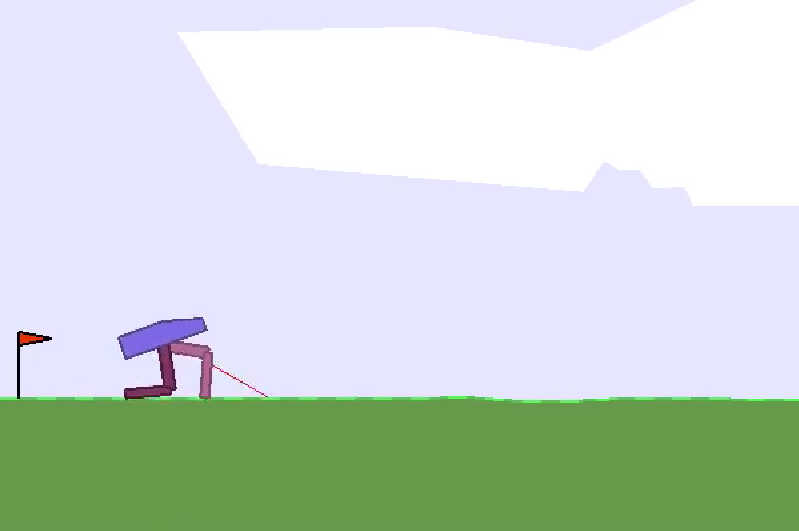
\includegraphics[width=0.9\linewidth]{figures/bipedal/classic.png}
		\caption{BipedalWalker-v3 Snapshot~\cite{noauthor_bipedalwalker-v2_2021}}
		\label{fig:bipedal_walker_classic}
	\end{subfigure}
	\begin{subfigure}{.5\textwidth}
		\centering
		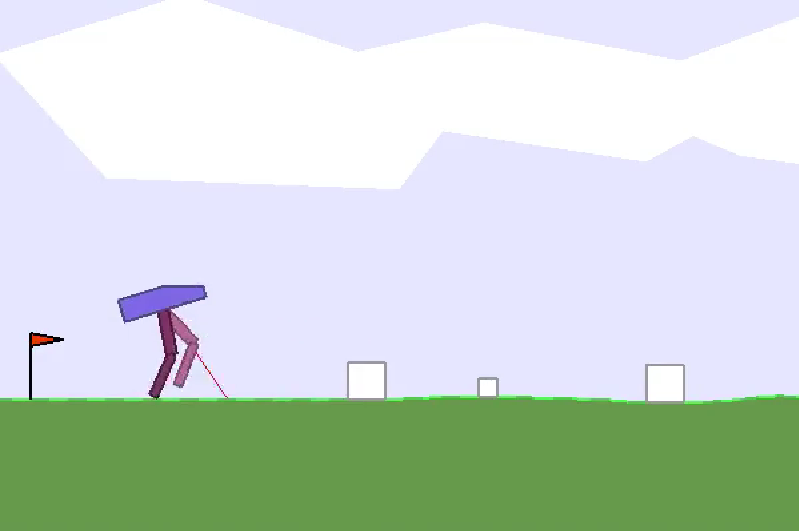
\includegraphics[width=0.9\linewidth]{figures/bipedal/hardcore.png}
		\caption{BipedalWalkerHardcore-v3 Snapshot~\cite{noauthor_bipedalwalkerhardcore-v2_2021}}
		\label{fig:bipedal_walker_hardcore}
	\end{subfigure}
	\caption{Bipedal Walkers Snapshots}
	\label{fig:bipedal_walkers}
\end{figure}

Locomotion of the Bipedal Walker is a difficult control problem due to following reasons: 
\begin{description}
	\item[Nonlinearity]. The dynamics are nonlinear, unstable and multimodal. 
	Dynamical behavior of robot changes for different situations 
	like ground contact, single leg contact and double leg contact.
	\item[Uncertainity]. The terrain where the robot walks may vary. 
	Designing a controller for all types of terrain is difficult.
	\item[Reward Sparsity]. Overcoming some obstacles requires a specific maneuver, which is hard to explore sometimes.	
	\item[Partially Observability]. The robot observes 
	ahead of it with lidar measurements and cannot observe behind. 
	In addition, it lacks of acceleration sensors.
\end{description}

These reasons make it hard to implement analytical methods for control tasks. 
However, approach can easily overcome nonlinearity and uncertainity problems.

On the other hand, reward sparsity problem brings local minimums to objective function of optimal control. It can be solved by a good exploration strategy and reward shaping. 

For the partial observability problem, more elegant solution is required. 
This is achieved by creating a belief state from the past observations to inform the agent. 
Agent uses this belief state to choose how to act. 
If belief state is evaluated sufficiently, 
this increases performance of the agent.
However, relying on observations is also possible, 
and this may be enough sometimes if advanced type of control is not required. 

\subsection{Deep Learning Library: PyTorch}
\label{dl_pytorch}
PyTorch is an open source library developed by Facebook's AI Research Lab (FAIR)~\cite{paszke_pytorch_2019}. 
It is based on Torch library~\cite{collobert_torch7_2011} and has Python and C++ interface. 
It is an automatic differentation library with accelerated mathematical operations backed by graphical processing units (GPUs). 
The clean pythonic syntax made it most famous deep learning tool among researches. 

\section{Proposed Methods and Contribution}
\label{sec:proposed_methods}

Partially observable environments are always a hard work for reinforcement learning algorithms. 
In this work, the walker environment assumed as fully observable environment at first. 
A Residual Feed-Forward Neural Network architecture is proposed to control 
the robot under fully observability assumption since no memory is used during decision making. 
Then, the environment is assumed to be partially observable. 
In order to recover belief states, Long Short Term Memory (LSTM) and 
Transformer neural networks are proposed using fixed number of 
last observations (4 in our case) during decision making. 

LSTMs are used in many deep learning applications which includes sequential data. 
It is a variant of Recurrent Neural Networks (RNN). 
It is a good candidate for RL algorithms which solves partially observable environments. 

Transformers are developed to handle sequential data as RNN models does. 
However, it processes the whole sequence at same time, while RNNs process the sequence in order. 
It replaced RNNs in Natural Language Processing (NLP) tasks over RNNs due to its major improvements. 
However, this is not the case for Reinforcement Learning, yet.

In order to handle reward sparsity problem, reward function is reshaped. Also, a exploration strategy is formed such that agent both explores and learns well. 

As RL algorithm, Twin Delayed Deep Deterministic Policy Gradient (TD3) and Soft Actor Critic (SAC) is used. TD3 is improved version of Deep Deterministic Policy Gradient (DDPG) Algorithm. And SAC is stochastic type of RL method which encourages agent to explore without explicit exploration definition.

\section{Related Work}
\label{sec:related_work}

Reinforcement Learning methods are used in many mechanical control tasks 
such as autonomus driving \cite{pan_virtual_2017, shalev-shwartz_safe_2016, sallab_deep_2017, wang_deep_2019} 
and autonomus flight \cite{kopsa_reinforcement_2018, abbeel_application_2006, santos_experimental_2012}.

Rastogi \cite{rastogi_deep_2017} used Deep Deterministic Policy Gradient (DDPG) algorithm to walk 
their physical bipedal walker robot along with simulation environment. 
They concluded that DDPG is infeasible to control walker robot 
since it requires long time for convergence. 
Kumar et al. \cite{kumar_bipedal_2018} also used DDPG to perform 
robot walking in 2D simulation environment. 
Their agent converged in approximately 25,000 episodes. 
Song et al. \cite{song_recurrent_2018} pointed out the partial observability problem of bipedal walker, 
using Recurrent Deep Deterministic Policy Gradient (RDDPG)~\cite{heess_memory-based_2015} algorithm 
and acquired better results than original Deep Deterministic Policy Gradient (DDPG) algorithm. 
Haarnoja et al. \cite{haarnoja_learning_2019} used maximum entropy learning for gaiting of real robot and achieved stable gait in 2 hours. 

Fris \cite{fris_landing_2020} used Twin Delayed Deep Deterministic Policy Gradient (TD3) 
using LSTM for their quadrocopter landing task. 
Fu et al. \cite{fu_when_2020} used vanilla RNN with attention mechanism 
using TD3 for car driving task, but not explicit Transformer. 
They reported that their method outperformed 7 baselines. 
Upadhyay et al. \cite{upadhyay_transformer_2019} used all of feed forward network, 
LSTM an original Transformer architectures for balancing pole 
on a cart from Cartpole environment of Gym, and Transformer yield worst results among three architectures.

\section{Outline of the Thesis}
\label{sec:outline}
This thesis consists of five main chapters. 
In Chapter 2, we discuss the theory of Reinforcement Learning and introduce the methods used in this thesis.
In Chapter 3, we explained the theory of Neural Networks and Deep Learning along with architectures which are designed to process sequential data. 
In Chapter 4, Bipedal Walker environments are presented, neural networks and RL algoritmhs are proposed, results are summarized and discussed.
In last Chapter, thesis is concluded by discussing obtained results and possible future works are discussed along with the future of RL.

\chapter{INTRODUCTION}
\label{chap:intro}

Artificial intelligence is the ability of a computer program 
or a machine to think and learn like natural intelligence 
performed by humans and animals. 
One way is to create an intellgent agent is using pattern detection  methods on data and use it to make predictions on unseen data. 
This approach is called Machine Learning. 

Humans and animals exhibit several different behaviours in terms of 
interaction with environment, such as utterance and movement. 
Their behavior is based on past experience, the situation they are in  and their objective. 
Like humans and animals, an intelligent agent is expected to take 
action according to its perception based some objective. 
A major challenge to machine learning is creating agents that will 
act more natural and humanlike. 
As a subfield of Machine Learning, Reinforcement Learning allows an 
agent to learn how to control (or act) itself in different situations by interaction with environment. 
In RL, environment is modeled to give reward or punishment to agent 
according to environmental state and agent actions, and agent focuses
on learning to predict what actions will lead to highest reward 
(or lowest punishment, based on its objective) in the future using past experience. 

Traditional RL algorithms need feature engineering from observation. 
For complex problems, the way to extract features is ambiguous or 
observations are not enough to create a good model. 
As a newer  technique, deep neural networks allows to extract 
high level features from data with large state-space 
(pixelwise visual, many kinematic sensors etc.) and missing  observations. 
Along with recent developments in DNNs, Deep Reinforcement Learning 
allows an agent to interact with environment in more complex way. 
DRL is based on neural networks which are function approximators. 
The problem with DRL is selection of a correct neural network, 
but there is still no analytical method to design a neural network for a particular task. 
Therefore, neural design is commonly based on trial-error. 

Since its discovery, robots have been crucial devices for the human race, whether smart or not. 
Intelligent humanoid and animaloid robots have been in 
continuous development since early 1980s. 
This type of robots has legs unlike driving robots. 
Since most of world terrain is unpaved, this type of robots are good alternative to driving robots. 
Locomotion is major task for such robots. Stable bipedal (2 legged)  walking 
is one of the most challenging problem among the control problems. 
It is hard to create accurate model due to high order of dynamics,  friction and discontinuities. 
Even so, design of walking controller using traditional methods is difficult due to same reasons. 
Therefore, for bipedal walking, DRL approach is an easier choice if a simulation environment is available. 

In this thesis, Bipedal Locomotion Deep Reinforcement Learning (DRL) by is investigated through \textit{BipedalWalker-Hardcore-v3} \cite{noauthor_bipedalwalkerhardcore-v2_2021} environment of open source GYM library \cite{brockman_openai_2016}. Different neural architectures are used and results are compared. 

\section{Reinforcement Learning and Optimal Control}
\label{sec:rl_and_control}
Optimal control is a field of mathematical optimization, concerned by  finding control policy of a dynamical system (environment) for given objective. For example, objective might be total reveune for a company as system, minimal fuel burn for a car as system, or total production for a factory. \\
RL is kind of naive subfield of Optimal Control. However, RL algorithms find policy (controller) by error minimization of objective from experience, while Optimal Control methods are concerned exact analytical optimal solutions based on dynamic model of environment and agent. \\
Optimal Control methods are efficient and robust when mathematical model of environment is available, accurate enough and solvable for optimal controller. However, some real world problems usually do not exhibit all of these conditions. In such cases, Reinforcement Learning is an easier way to derive a control policy.

\section{Challenges}
\label{sec:chal}

The Reinforcement Learning Environment poses a variety of obstacles 
that we need to address and potentially make trade-offs among them~\cite{dulac-arnold_challenges_2019, sutton_reinforcement_1998}.

\subsection{Exploration Explotation Dilemma}

A RL agent is supposed to maximize rewards (knowledge exploration) by observing the environment (exploration of environment). 
This gives rise to the exploration-exploitation dilemma that is the inevitable trade-off between them. 
Exploration is taking a range of acts to benefit about the consequences. 
Typically results in low immediate rewards and high rewards for the future. 
Explotation is taking action that has been learned. Typically results in high immediate rewards and low rewards in the future. 

\subsection{Generalization and Curse of Dimensionality}

A RL agent should also be able to generalize experiences to act on unseen situation before. 
This issue arises when state space and action space is high dimensional since experiencing all possibilities is impractical. 
This is solved by introducing function approximator. Deep Reinforcement Learning uses neural network as function approximator. 

\subsection{Delayed Consequences}

A RL agent should be aware reason of reward or punishment. 
Once it gets reward or punishment, it should be able to discriminate whether reward is caused by instant actions or past actions. 

\subsection{Partial Observability}

Partial observability is absence of all required observation to infer instant state. 
For instance, a driver does not know engine temperature or rotational speed of gears. 
Although driver is able to drive in that case, s/he would not be able to drive well on traffic in absence of rear view mirror or side mirror. 
In real world, most of systems are partially observable. 
This problem is usually tackled by incorprating observation history from agents memory in acting. 

\subsection{Safety of Agent}

Mechanical agents can kill or degrade themselves and their surroundings. 
This safety problem is important on both exploration stage and full operation. 
Simulation of environment is a good way to train agent with safety but causes incomplete learning 
due to inaccuracy compared to real environment. 

\section{Sequential Decision Making}
\label{sec:decision_making}

RL is a stochastic control process in discrete time~\cite{sutton_reinforcement_1998}. 
At time $t$, the agent starts with state $s_t$ and observes $o_t$, 
then takes action $a_t$ according to its policy $\pi$ and obtains reward $r_t$ at time $t$. 
Then state transition to $s_{t+1}$ occurs as a consequence of action and agent observes next observation $o_{t+1}$. 
History is set of past actions observations and rewards, $h_t=\{ a_0, o_0, r_0, ... a_t, o_t, r_t\}$. 
State $s_t$ is a function of the history, $s_t=f(h_t)$, which represents situation of environment as much as possible. 
The RL diagram is visualized in \figref{fig:rl_diagram}. 
\begin{figure}
	\centering
	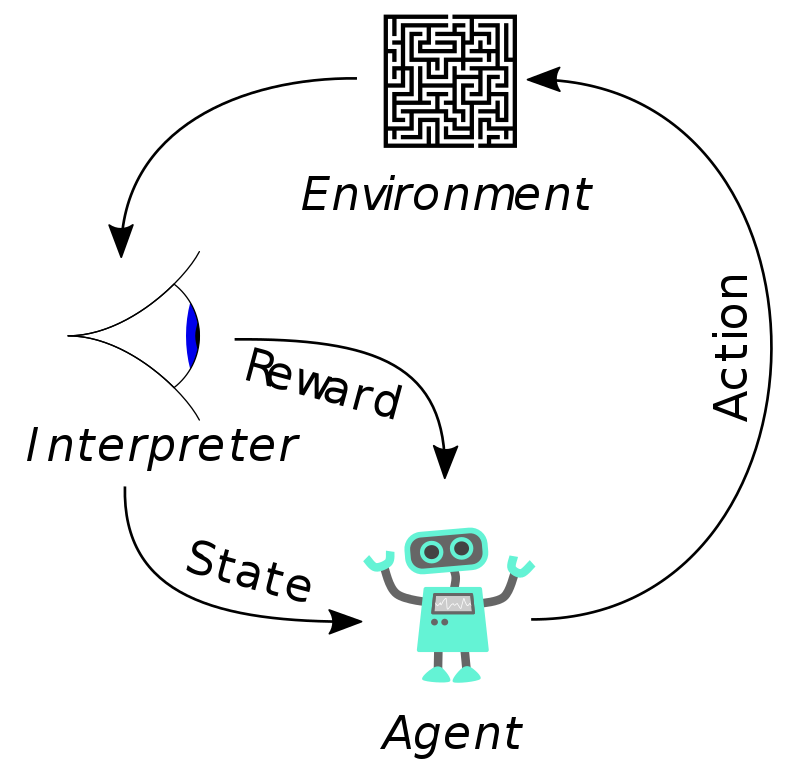
\includegraphics[width=0.7\textwidth]{figures/ml_theory/RL_diagram.png}
	\caption{Reinforcement Learning Diagram}
	\label{fig:rl_diagram}
\end{figure}
\section{Markov Decision Process}
\label{sec:mdp}

Markov Decision Process (MDP) is a control process with reward function and discount factor. It is represented as a tuple $(S,A,P,R,\gamma)$. Markov property means that the conditional probability distribution of the future state depends only on the instant state and action instead of the entire past. 

\textbf{State}: State $s \in S$

\textbf{Acgtion}: Action $s \in S$

\textbf{Model}: Model is mathematical representation of how environment evolves through time, including transition probabilities $p(s'|s,a)$ where $s' \in S$ is next state, $s \in S$ is instant state and $a \in A$ is taken action.

\textbf{Reward}: Reward $R \colon S \times A \mapsto \mathbb{R}$ is a function of state and action. It is ultimate utility function of Reinforcement Learning.

\textbf{Discount Factor and Return}: xxx Horizon?

\textbf{Policy}: It is a mapping $\pi \colon S \mapsto A$ which maps states to actions. 

\subsection{Value Functions}

\subsubsection{State Value Function}

\subsubsection{State-Action Value Function}

\section{Partially Observed Markov Decision Process}
\label{sec:pomdp}

In MDP, agent observes states as it is. 
However, observation space is not enough to represent all information (state) about environment sometimes. 
In such cases, past and instant observations are used to filter out a belief state. 
It is represented as a tuple $(\mathcal{S},\mathcal{A},T,R,\mathcal{O},O,\gamma)$. 
In addition to MDP, it introduces observation space $\mathcal{O}$ and observation model $O$ \cite{francois-lavet_introduction_2018}. 

\begin{description}
	\item[Observation Space $\mathcal{O}$] A set of all possible observations of agent.
	\item[Observation Model $O \colon \mathcal{O} \times \mathcal{S} \mapsto \lbrack 0,1 \rbrack$] Function of how observations are related to states, 
	representing observation probabilities as $O(o|s) = p(o|s)$ 
	where $s \in \mathcal{S}$ is instant state and $o \in \mathcal{O}$ is observation.
\end{description}

Since states are not observed directly, agent must use observations while deriving a control policy. 
\section{Policy and Control}
\label{sec:policy_control}

\subsection{Policy}

A policy defines how the agent acts according to the state of the environment. 
It may be either deterministic or stochastic: 

\begin{description}
	\item[Deterministic Policy $\mu \colon \mathcal{S} \rightarrow \mathcal{A}$] 
	A mapping from states to actions.
	\item[Stochastic Policy $\pi \colon \mathcal{S} \times \mathcal{A} \rightarrow \lbrack 0,1 \rbrack$] 
	A mapping from state-action pair to a probability value.
\end{description}

\subsection{Return}

At time $t$, return $G_t$ is a cumulative sum of the future rewards scaled by the discount factor $\gamma$: 
\begin{equation}
\label{eqn:return_dfn}
G_t = \sum_{i=t}^{\infty} \gamma^{i-t} r_i = r_t + \gamma G_{t+1}.
\end{equation}
Since the return depends on future rewards, it also depends on the  policy of the agent as it affects the future rewards.

\subsection{State Value Function}

State Value Function $V^{\pi}$ is the expected return when policy $\pi$ is followed in the future and is defined by
\begin{equation}
V^{\pi}(s) = \mathbb{E}[G_t|s_t=s, \pi]. % \quad \forall t = 0,1, ...
\end{equation}
Optimal value function should return maximum expected return, where 
the behavior is controlled by the policy. 
In other words, 
\begin{equation}
\label{eqn:max_v}
V^{*}(s) = \max_{\pi} V^{\pi}(s).
\end{equation}

\subsection{State-Action Value Function}

State-Action Value Function $Q^{\pi}$ is again the expected return when policy $\pi$ is followed in the future, 
however, any action taken at the instant step:
\begin{equation}
Q^{\pi}(s,a) = \mathbb{E}[G_t|s_t=s, a_t=a, \pi]. %\quad \forall t = 0,1, ...
\end{equation}
Optimal state-action value function should yield maximum expected return for each state-action pair. Hence,
\begin{equation}
\label{eqn:max_q}
Q^{*}(s,a) = \max_{\pi} Q^{\pi}(s,a).
\end{equation}
The optimal policy $\pi^*$ can be obtained by $Q^{*}(s,a)$. For stochastic policy, it is defined as  
\begin{equation}
\label{eqn:policy_stochastic_q}
\pi^{*}(a|s) = 
\begin{cases}
1,   & \text{if  } a = \arg\max_{a} Q^{*}(s,a), \\
0,   & \text{otherwise  }.
\end{cases} 
\end{equation}
For deterministic policy, it is
\begin{equation}
\label{eqn:policy_deterministic_q}
\mu^{*}(s) = \arg\max_{a} Q^{*}(s,a).
\end{equation}

\subsection{Bellman Equation}

Bellman proved that optimal value function, for a model $T$, should satisfy following conditions~\cite{bellman_dynamic_2003}: 
\begin{equation}
\label{eqn:bellman_v}
V^{*}(s) = \max_{a} \Big\{ R(s,a) + \gamma \sum_{s'} T(s'|s,a) V^{*}(s') \Big\}
\end{equation}
\begin{equation}
\label{eqn:bellman_q}
Q^{*}(s,a) = R(s,a) + \gamma \max_{a'} \Big\{ \sum_{s'} T(s'|s,a) Q^{*}(s',a') \Big\}
\end{equation}
These equations can simply be derived from \eqref{eqn:max_v} and \eqref{eqn:max_q}. 
Most of RL methods are build upon solving \eqref{eqn:bellman_q}, since there exist a direct relation between $Q$ and $\pi$ as in \eqref{eqn:policy_deterministic_q} and \eqref{eqn:policy_stochastic_q}.

\section{Model-Free Reinforcement Learning}
\label{sec:mf_rl}

Model based methods are based on solving Bellman equation \eqref{eqn:bellman_v}, \eqref{eqn:bellman_q} with a given model $T$. 
On the other hand, Model-Free Reinforcement Learning is suitable 
if environment model is not available but the agent can experience environment by the consequences of its actions. There are three main categories in model-free RL:  

\begin{description}
	\item[Value-Based Learning] The value functions are learned, 
	hence the policy arises naturally from the value function using  \eqref{eqn:policy_stochastic_q} and \eqref{eqn:policy_deterministic_q}. 
	Since $\argmax$ operation is used, this type of learning is suitable for problems where action space is discrete. 
	
	\item[Policy-Based Learning] The policy is learned directly, 
	and return values are used instead of learning a value function. 
	Unlike value-based methods, it is suitable when continuous action spaces are available in the environment. 
	
	\item[Actor-Critic Learning] Both policy (actor) and value (critic) functions are learned simulatenously. 
	Thus, it is also suitable for continuous action spaces. 
	
\end{description}

\subsection{Q Learning}
Q Learning is a value-based type of learning. 
It is based on optimizing $Q$ function using Bellman Equation \eqref{eqn:bellman_q}~\cite{watkins_technical_1992}. 
In this learning strategy, $Q$ function is assumed to be parametrized by $\theta$. 
Target $Q$ value is estimated by bootstrapping estimate, 
\begin{equation}
\label{eqn:q_target}
Y_t^Q = r_t + \gamma \max_{a'} Q(s_{t+1},a';\theta).
\end{equation}
At time $t$,  with state, action, reward, next state tuples ($s_t,a_t,r_t,s_{t+1}$), 
$Q$ values are updated by minimizing difference between the target value and the estimated value.
Hence the loss 
\begin{equation}
\label{eqn:q_loss}
\mathcal{L}_t(\theta) = \big( Y_t - Q(s_t,a_t;\theta) \big) ^ 2, 
\end{equation}
is to be minimized with respect to $\theta$ using numerical optimization methods. 

\subsubsection{Deep Q Learning}
When a nonlinear approximator is used for $Q$ estimation, learning is unstable due to the correlation among recent observations, hence correlations between updated $Q$ function and observations.
Deep Q Learning solves this problem by introducing Target Network and Experience Replay \cite{mnih_human-level_2015, mnih_playing_2013} along with using deep neural networks. 

\textbf{Target Network} is parametrized by $\theta^-$. 
It is used to evaluate target value, but it is not updated by the loss minimization. 
It is updated at each fixed number of update step by Q network parameter $\theta$. 
In this way, correlation between target value and observations are reduced.
The target value is obtained by using $\theta^-$ as
\begin{equation}
\label{eqn:dqn_ntarget}
Y_t^{DQN} = r_t + \gamma \max_{a'} Q(s_{t+1},a';\theta^-).
\end{equation}

\textbf{Experience Replay} stores experience tuples in the replay memory $\mathcal{D}$ as a queue with fixed buffer size $N_{replay}$. 
At each iteration $i$, $\theta$ is updated by experiences $(s,a,r,s')\sim U(\mathcal{D})$ uniformly subsampled from experience replay by minimizing the expected loss
\begin{equation}
\label{eqn:dqn_loss}
\mathcal{L}_i(\theta_i) = \mathbb{E}_{(s,a,r,s')\sim U(\mathcal{D})}\Big[\big( Y^{DQN} - Q(s,a;\theta_i) \big) ^ 2 \Big].
\end{equation}
It allows agent to learn from experiences multiple times at different stages of learning. 
More importantly, sampled experiences are close to be independent and identically distributed if buffer size is large enough. 
Again, this reduces correlation between recent observations and updated $Q$ value. This makes learning process more stable. 

\textbf{Epsilon Greedy Exploration} is used to let agent explore environment. 
In discrete action space (finite action space $\mathcal{A}$), this is 
the simplest exploration strategy used in RL algorithms.
During the learning process, a random action with probability $\epsilon$ is selected or greedy action (maximizing Q value) with probability $1-\epsilon$. In order to construct policy:   
\begin{equation}
\label{eqn:egreedy_policy}
\pi(a|s) = 
\begin{cases}
1-\epsilon,   & \text{if } a = \argmax_{a} Q(s, a), \\
\frac{\epsilon}{|\mathcal{A}|-1},     & \text{otherwise},
\end{cases}
\end{equation}
where $|\mathcal{A}|$ denotes cardinality of $\mathcal{A}$. 
In Algorithm~\ref{alg:dqn}, we summarize the Deep Q Learning with Experience Replay. 

\begin{algorithm}[H]
	\SetAlgoLined
	\DontPrintSemicolon % Some LaTeX compilers require you to use \dontprintsemicolon instead
	Initialize: $\mathcal{D}$, $N$, $N_{replay}$, $\theta$, $\epsilon$, $d$ \\
	$\theta^- \leftarrow \theta$ \\
	\For{$\text{episode} = 1, M $}{
		Recieve initial state $s_1$; \\
		\For{$t = 1, T$}{
			Randomly select action $a_t$ with probability $\epsilon$, otherwise $a_t = \arg\max_{a} Q(s_t, a; \theta)$ greedily; \\
			Execute action $a_t$ and recieve reward $r_t$ and next state $s_{t+1}$; \\
			Store experience tuple $e_t = (s_t, a_t, r_t, s_{t+1})$ to $\mathcal{D}$ ; \\
			Sample random batch $\mathcal{D}_{r}$ ($|\mathcal{D}_{r}|=N$) from $\mathcal{D}$; \\
			$Y_j = \begin{cases}
			r_j & \text{if } s_{j+1} \text{ terminal } \\
			r_j + \gamma \max_{a'} Q(s_{j+1},a';\theta^-) & \text{otherwise } 
			\end{cases}$ \qquad $\forall e_j \in \mathcal{D}_{r}$\\
			Update $\theta$ by minimizing $ \frac{1}{N}\sum_{e_j \in \mathcal{D}_{r}} \big[ Y_j - Q(s_j,a_j;\theta) \big] ^ 2$ for a single step; \\
			\lIf{$t \mod d$}{
				Update target network: $\theta^- \leftarrow \theta$;
			}
		}
	}
	\caption{Deep Q Learning with Experience Replay}
	\label{alg:dqn}
\end{algorithm}

\subsubsection{Double Deep Q Learning}
In DQN, maximum operator is used to both select and evaluate action on the same network as in \eqref{eqn:dqn_ntarget}. 
This yields overestimation of $Q$ function in noisy environments. 
Therefore, action selection and value estimation is decoupled in target evaluation to overcome $Q$ function overestimation~\cite{van_hasselt_deep_2015} using Double Deep Q Network (DDQN). 
The target value in this approach can therefore be written as follows:
\begin{equation}
\label{eqn:ddqn_ntarget}
Y_t^{DDQN} = r_t + \gamma Q(s_{t+1}, \arg\max_{a'} Q(s_{t+1}, a'; \theta_i );\theta^-).
\end{equation}
Except the target value, the learning process is the same as in DQN. 

\subsection{Actor-Critic Learning}

Value-based methods are not suitable for continuous action spaces. 
Therefore, policy should be explicitly defined instead of maximizing $Q$ function. 
For such problems, actor-critic type learning methods use both value and policy models seperately. 

In actor-critic learning, there exists two components~\cite{silver_deterministic_2014}:  
First one is the actor, which is the policy function, either stochastic or deterministic, parametrized by $\theta^{\pi}$ or $\theta^{\mu}$, respectively. 
For policy learning, an estimate of the value function is used instead of the true value function since it is already unknown. 
Second one is the critic, which is an estimator of the $Q$ value, parametrized by $\theta^Q$. 
Critic learning is achieved by minimizing the error obtained by either Monte Carlo sampling or Temporal Difference bootstrapping.
Critic is what policy uses for value estimation. 

The ultimate goal is to learn a policy maximizing the value function $V$ by selecting action which maximizes $Q$ value in \eqref{eqn:policy_deterministic_q}. 
Therefore, value function is the criteria to be maximized by solving parameters $\theta^\pi$ (or $\theta^\mu$) given $\theta^Q$. 
At time $t$, the loss function for the policy is negative, that is,  
\begin{equation}
\label{eqn:ac_value_maximization}
\mathcal{L}_t(\theta^\pi) = - Q(s_t, \widetilde{a}_t;\theta^Q), \quad \widetilde{a}_t \sim \pi(\cdot|s_t;\theta^\pi).
\end{equation}

In order to learn policy $\pi$, $Q$ function should also be learned simultaneously. 
For $Q$ function approximation, the target value is parametrized by $\theta^Q$ and $\theta^\pi$,
\begin{equation}
\label{eqn:ac_target}
Y_t^{AC} = r_t + \gamma Q(s_{t+1}, \widetilde{a}_{t+1};\theta^Q), \quad \widetilde{a}_{t+1} \sim \pi(\cdot|s_{t+1};\theta^{\pi}),
\end{equation}
and this target is used to learn $Q$ function by minimizing the least squares loss (in general),
\begin{equation}
\label{eqn:ac_loss}
\mathcal{L}_t(\theta^Q) = \big[ Y_t^{AC} - Q(s_t,a_t;\theta^Q) \big] ^ 2.
\end{equation}

Note that both the actor and the critic should be learned at the same time. Therefore, parameters are updated simultaneously during the iterations in the learning process. 

\subsubsection{Deep Deterministic Policy Gradient}
DDPG is continuous complement of DQN using a deterministic policy~\cite{lillicrap_continuous_2019}. 
It also uses experience replay and target networks. 
Similar to Deep Q Learning, there are target networks parametrized by $\theta^{\mu^-}$ and $\theta^{Q^-}$ 
along with the main networks parametrized by $\theta^{\mu}$ and $\theta^{Q}$. 

While target networks are updated in a fixed number of steps in DQN, 
DDPG updates target network parameters at each step with Polyak averaging, 
\begin{equation}
\label{eqn:target_update}
\theta^- \leftarrow \tau \theta + (1-\tau) \theta^- .
\end{equation}
The $\tau$ is an hyperparameter indicating how fast the target network is updated and it is usually close to zero. 

Policy network parameters are learned by maximizing resulting expected value, or minimizing its negative,
\begin{equation}
\label{eqn:ddpg_policy_loss}
\mathcal{L}_i(\theta^\mu_i) = -\mathbb{E}_{s \sim U(\mathcal{D})} \Big[ Q(s, \mu(s\theta^\mu_i);\theta^Q) \Big].
\end{equation} 
Note that value network parameters are also assumed to be learned. 

In addition, target networks are used to predict target value and the target is defined by
\begin{equation}
\label{eqn:ddpg_target}
Y_t^{DDPG} = r_t + \gamma Q(s_{t+1}, \mu(s_{t+1};\theta^{\mu^-});\theta^{Q^-}).
\end{equation}
In each iteration, this target is used to learn $Q$ function by minimizing the least squares loss 
\begin{equation}
\label{eqn:ddpg_loss}
\mathcal{L}_i(\theta^Q_i) = \mathbb{E}_{s,a,r,s'\sim U(\mathcal{D})}\Big[\big( Y^{DDPG} - Q(s,a;\theta^Q_i) \big) ^ 2 \Big].
\end{equation}

In DDPG, value and policy network parameters are learned simultaneously. 
During the learning process, exploration noise is added to each selected action, sampled by a process $\mathcal{X}$. 
In ~\cite{lillicrap_continuous_2019}, authors proposed to use Ornstein-Uhlenbeck Noise~\cite{uhlenbeck_theory_1930} in order to have temporal correlation for efficiency. 
However, a simple Gaussian white noise or any other one is also possible. 

DDPG is summarized in Algorithm \ref{alg:ddpg}. 

\begin{algorithm}[H]
	\SetAlgoLined
	\DontPrintSemicolon % Some LaTeX compilers require you to use \dontprintsemicolon instead
	Initialize: $\mathcal{D}$, $N$, $N_{replay}$, $\theta^{\mu}$, $\theta^Q$, $\mathcal{X}$ \\
	$\theta^{\mu^-} \leftarrow \theta^{\mu}$, $\theta^{Q^-} \leftarrow \theta^{Q}$ \\
	\For{$\text{episode} = 1, M $}{
		Recieve initial state $s_1$; \\
		\For{$t = 1, T$}{
			Select action $a_t = \mu(s_t; \theta^{\mu}) + \epsilon$ where $\epsilon \sim \mathcal{X}$; \\
			Execute action $a_t$ and recieve reward $r_t$ and next state $s_{t+1}$; \\
			Store experience tuple $e_t = (s_t, a_t, r_t, s_{t+1})$ to $\mathcal{D}$ ; \\
			Sample random batch $\mathcal{D}_{r}$ ($|\mathcal{D}_{r}|=N$) from $\mathcal{D}$; \\
			$Y_j = \begin{cases}
			r_j & \text{if } s_{j+1} \text{ terminal } \\
			r_j + \gamma Q(s_{j+1},\mu(s_{j+1}; \theta^{\mu^-}); \theta^{Q^-}) & \text{otherwise }
			\end{cases}$ \qquad $\forall e_j \in \mathcal{D}_{r}$ \\
			Update $\theta^Q$ by minimizing $ \frac{1}{N}\sum_{e_j \in \mathcal{D}_{r}} \big( Y_j - Q(s_j,a_j;\theta^Q) \big) ^ 2$ for a single step; \\
			Update $\theta^{\mu}$ by maximizing $ \frac{1}{N}\sum_{e_j \in \mathcal{D}_{r}} Q(s_j,a_j;\theta^Q)$ for a single step; \\
			Update target networks: \\
			$\theta^{\mu^-} \leftarrow \tau \theta^{\mu} + (1-\tau) \theta^{\mu^-}$ and \\
			$\theta^{Q^-} \leftarrow \tau \theta^{Q} + (1-\tau) \theta^{Q^-}$;
		}
	}
	\caption{Deep Deterministic Policy Gradient}
	\label{alg:ddpg}
\end{algorithm}

\textbf{Ornstein-Uhlenbeck Process} is the continuous analogue of the discrete first order autoregressive (AR(1)) process~\cite{uhlenbeck_theory_1930}. 
The process $x$ is defined by a stochastic differential equation,
\begin{equation}
\label{eqn:ou_process}
\frac{dx}{dt} = -\theta x + \sigma \eta(t),
\end{equation}
where $\eta(t)$ is a white noise. 
Its standard deviation in time is equal to $\frac{\sigma}{\sqrt{2\theta}}$. 
This process is commonly used as an exploration noise in physical environments since it has temporal correlation. 
Two sample paths of the process are shown in  \figref{fig:ou_vs_gaussian} in order to compare with the Gaussian noise.

\begin{figure}
	\centering
	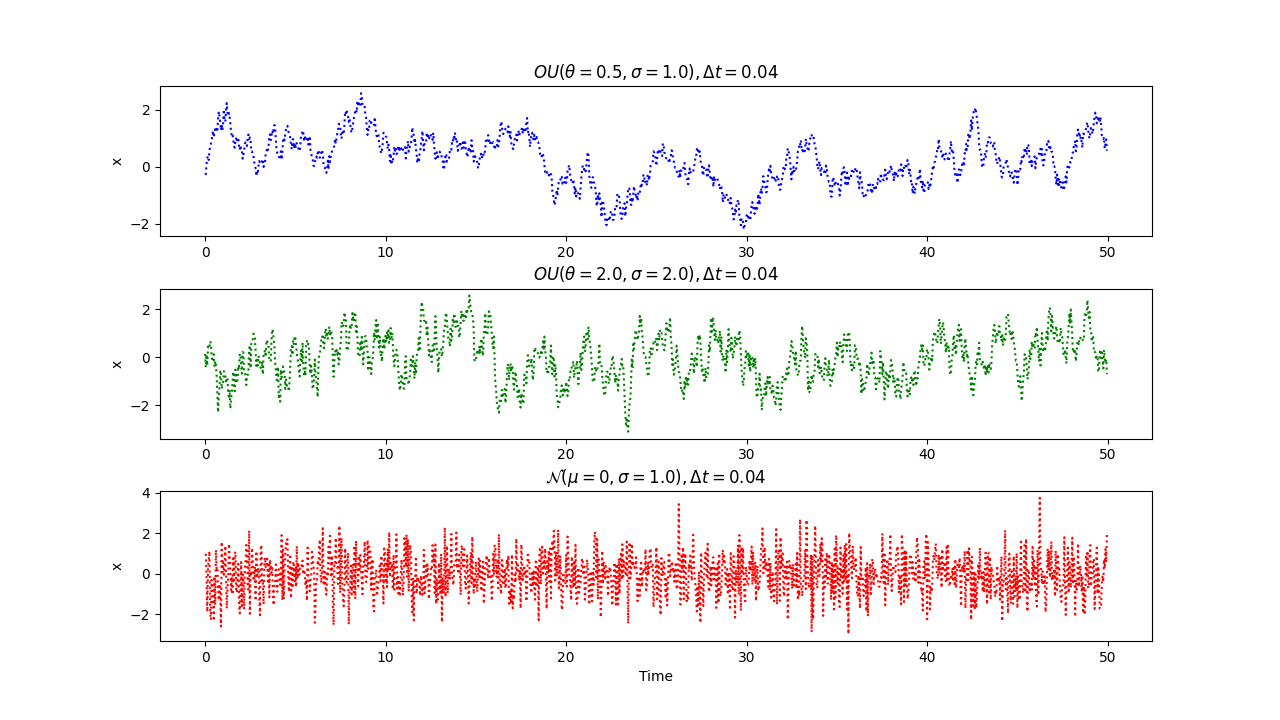
\includegraphics[width=0.98\textwidth]{figures/others/random_processes.png}
	\caption{Ornstein-Uhlenbeck Process and Gaussian Process comparison}
	\label{fig:ou_vs_gaussian}
\end{figure}

\subsubsection{Twin Delayed Deep Deterministic Policy Gradient}
TD3~\cite{fujimoto_addressing_2018} is an improved version of DDPG with higher stability and efficiency. 
There are three main tricks upon DDPG: 

\textbf{Target Policy Smoothing} is to regularize the learning process by smoothing effects of actions on value. For target value assessing, actions are obtained from the target policy network in DDPG, while a clipped zero-centered Gaussian noise is added to actions in TD3 as follows: 
\begin{equation}
\label{eqn:td3_target_action}
\widetilde{a}' = \mu(s';\theta^{\mu^-}) + \text{clip}(\epsilon, -c, c), \quad \epsilon \sim \mathcal{N}(0, \sigma^2).
\end{equation}

\textbf{Clipped Double Q Learning} is to escape from $Q$ value overestimation. 
There are two different value networks with their targets. 
During learning, both networks are trained by single target value assessed by using whichever of the two networks give smaller. 
In other words, 
\begin{equation}
\label{eqn:td3_target}
Y_t^{TD3} = r_t + \gamma \min_{k\in\{1,2\}} Q(s_{t+1}, ;\widetilde{a}_{j+1};\theta^{Q_k^-}).
\end{equation}
On the other hand, the policy is learned by maximizing the output of the first value network, or minimizing its negative,
\begin{equation}
\label{eqn:td3_policy_loss}
\mathcal{L}_i(\theta^\mu_i) = -\mathbb{E}_{s \sim U(\mathcal{D})} \Big[ Q(s, \mu(s;\theta^\mu_i);\theta^{Q_1}) \Big].
\end{equation} 

\textbf{Delayed Policy Updates} is used for stable training. 
During learning, policy network and target networks are updated less frequently (at each fixed number of steps) than the value network. 
Since the policy network parameters are learned by maximizing the value network, they are learned slower.  

TD3 is summarized in Algorithm \ref{alg:td3}. 

\begin{algorithm}[H]
	\SetAlgoLined
	\DontPrintSemicolon % Some LaTeX compilers require you to use \dontprintsemicolon instead
	Initialize: $\mathcal{D}$, $N$, $N_{replay}$, $\theta^{\mu}$, $\theta^Q_1$, $\theta^Q_2$, $\mathcal{X}$, $\sigma$, $c$, $d$ \\
	$\theta^{\mu^-} \leftarrow \theta^{\mu}$, $\theta^{Q^-}_1 \leftarrow \theta^{Q}_1$, $\theta^{Q^-}_2 \leftarrow \theta^{Q}_2$ \\
	\For{$\text{episode} = 1, M $}{
		Recieve initial state $s_1$; \\
		\For{$t = 1, T$}{
			Select action $a_t = \mu(s_t; \theta^{\mu}) + \epsilon$ where $\epsilon \sim \mathcal{X}$
			Execute action $a_t$ and recieve reward $r_t$ and next state $s_{t+1}$; \\
			Store experience tuple $e_t = (s_t, a_t, r_t, s_{t+1})$ to $\mathcal{D}$ ; \\
			Sample random batch $\mathcal{D}_{r}$ ($|\mathcal{D}_{r}|=N$) from $\mathcal{D}$; \\
			Sample target actions for value target,
			$\widetilde{a}_{j+1} = \mu(s_{j+1};\theta^{\mu^-}) + \text{clip}(\epsilon, -c, c), \quad \epsilon \sim \mathcal{N}(0, \sigma^2) \quad \forall e_j \in \mathcal{D}_{r}$; \\
			$Y_{jk} = \begin{cases}
			r_j & \text{if } s_{j+1} \text{ terminal } \\
			r_j + \gamma Q(s_{j+1},\widetilde{a}_{j+1}); \theta^{Q^-}_k) & \text{otherwise } 
			\end{cases}$ \qquad $\forall e_j \in \mathcal{D}_{r}$, $\forall k \in \{1,2\}$ \\
			$Y_j = \min(Y_{j1}, Y_{j2})$; \\
			Update $\theta^Q_1$ $\theta^Q_2$ by seperately minimizing $ \frac{1}{N}\sum_{e_j \in \mathcal{D}_{r}} \big( Y_j - Q(s_j,a_j;\theta^Q_k) \big) ^ 2 \quad \forall k \in \{1,2\}$ for a single step; \\
			\uIf{$t \mod d$}{
				Update $\theta^{\mu}$ by maximizing $ \frac{1}{N}\sum_{e_j \in \mathcal{D}_{r}} Q(s_j,a_j;\theta^Q_1)$ for a single step; \\
				Update target networks: \\
				$\theta^{\mu^-} \leftarrow \tau \theta^{\mu} + (1-\tau) \theta^{\mu^-}$ and \\
				$\theta^{Q^-}_k \leftarrow \tau \theta^{Q}_k + (1-\tau) \theta^{Q^-}_k \quad \forall k \in \{1,2\}$ ;
			}
		}
	}
	\caption{Twin Delayed Deep Deterministic Policy Gradient}
	\label{alg:td3}
\end{algorithm}

\subsubsection{Soft Actor-Critic}
SAC~\cite{haarnoja_soft_2018} is a stochastic actor-critic method and many characteristics are similar to TD3 and DDPG. Its main advantage is that it learns to maximize exploration with entropy regularization. 

SAC is an entropy-regularized RL method. Such methods give bonus reward to the agent propotional to the policy entropy: given state $s$, the entropy of a policy $\pi$ is defined by
\begin{equation}
\label{eqn:policy_entropy}
H(\pi(\cdot|s)) = \mathbb{E}_{\widetilde{a}\sim\pi(\cdot|s)}[-\log(\pi(\widetilde{a}|s))].
\end{equation}

Given the entropy coefficient $\alpha$, definition of state-action value function is redefined as follows: 
\begin{equation}
\label{eqn:q_dfn_entreg}
Q^{\pi}(s,a) = \mathbb{E}_{\substack{s'\sim T(\cdot|s,a)\\\widetilde{a}'\sim \pi(\cdot|s')} } \Big[r + \gamma \Big(Q^{\pi}(s',\widetilde{a}') -\alpha\log(\pi(\widetilde{a}'|s') \Big) \Big]. %\quad \forall t = 0,1, ...
\end{equation}

This modification changes $Q$ value target definition,
\begin{equation}
\label{eqn:q_target_sac}
Y_t^{SAC} = r_t + \gamma \Big(\min_{k\in\{1,2\}} Q(s_{t+1}, ;\widetilde{a}_{t+1};\theta^{Q_k^-}) -\alpha\log(\pi(\widetilde{a}_{t+1}|s_{t+1})) \Big),
\end{equation}
where $\widetilde{a}_{t+1} \sim \pi(\cdot|s_{t+1}; \theta^{\pi})$.

While the policy is updated according to first value network by \eqref{eqn:td3_policy_loss} in TD3, the policy is updated according to minimum value of both networks output along with the entropy regularization, 
\begin{equation}
\label{eqn:sac_policy_loss}
\mathcal{L}_i(\theta^\pi_i) = - \mathbb{E}_{\substack{s \sim U(\mathcal{D})\\\widetilde{a} \sim \pi(\cdot|s)}} \Big[ \min_{k\in\{1,2\}} Q(s, \widetilde{a};\theta^{Q_k^-}) - \alpha\log(\pi(\widetilde{a}|s;\theta^\pi_i)) \Big].
\end{equation}

The policy function is stochastic in SAC, and in practice, it is a parametrized probability disribution. Most common one is 
Squashed Gaussian policy to squash actions in the range $(-1,1)$ by $\tanh$ function. 
This is parametrized by its mean and standart deviation, i.e., $\theta^{\pi}=(\theta^{\mu}, \theta^{\sigma})$. Actions are then sampled as follows: 
\begin{equation}
\label{eqn:squashed_gp_sampling}
a(s) = \tanh(\mu(s; \theta^{\mu}) + \eta \odot \sigma(s; \theta^{\sigma})), \quad \eta \sim \mathcal{N}(0, I), 
\end{equation}
where $\odot$ is elementwise multiplication.

Finally, we note that SAC method does not include policy delay, target policy smoothing and target policy network. 

SAC is summarized in Algorithm \ref{alg:sac}.

\begin{algorithm}[H]
	\SetAlgoLined
	\DontPrintSemicolon % Some LaTeX compilers require you to use \dontprintsemicolon instead	
	Initialize: $\mathcal{D}$, $N$, $N_{replay}$, $\theta^{\pi}$, $\theta^Q_1$, $\theta^Q_2$, $\alpha$ \\
	$\theta^{Q^-}_1 \leftarrow \theta^{Q}_1$, $\theta^{Q^-}_2 \leftarrow \theta^{Q}_2$ \\
	\For{$\text{episode} = 1, M $}{
		Recieve initial state $s_1$; \\
		\For{$t = 1, T$}{
			Select action $a_t \sim \pi(\cdot|s_t; \theta^\pi)$
			Execute action $a_t$ and recieve reward $r_t$ and next state $s_{t+1}$; \\
			Store experience tuple $e_t = (s_t, a_t, r_t, s_{t+1})$ to $\mathcal{D}$ ; \\
			Sample random batch with $N$ transitions from $\mathcal{D}$ as $\mathcal{D}_{r}$; \\
			Sample next actions for value target
			$\widetilde{a}_{j+1} \sim \pi(\cdot|s_{j+1};\theta^{\pi}) \quad \forall e_j \in \mathcal{D}_{r}$; \\
			$Y_{jk} = \begin{cases}
			r_j & \text{if } s_{j+1} \text{ terminal } \\
			r_j + \gamma \Big(Q(s_{j+1},\widetilde{a}_{j+1}; \theta^{Q^-}_k) - \alpha\log(\widetilde{a}_{j+1} | s_{j+1}; \theta^\pi)\Big) &  \text{otherwise }
			\end{cases}$ \qquad $\forall e_j \in \mathcal{D}_{r}$ $\forall k \in \{1,2\}$ \\
			$Y_j = \min(Y_{j1}, Y_{j2})$; \\	
			Update $\theta^Q_1$ $\theta^Q_2$ by seperately minimizing $ \frac{1}{N}\sum_{e_j \in \mathcal{D}_{r}} \big( Y_j - Q(s_j,a_j;\theta^Q_k) \big) ^ 2 \quad \forall k \in \{1,2\}$ for a single step; \\
			Sample actions for policy update,
			$\widetilde{a}_j \sim \pi(\cdot|s_j;\theta^{\pi}) \quad \forall e_j \in \mathcal{D}_{r}$; \\		
			Update $\theta^\pi$ by maximizing $ \frac{1}{N}\sum_{e_j \in \mathcal{D}_{r}} [\min_{k\in\{1,2\}} Q(s_j,\widetilde{a}_j;\theta^{Q_k})-\alpha\log(\pi(\widetilde{a}_j|s_j;\theta^\pi))]$ for a single step; \\
			Update target networks: \\
			$\theta^{Q^-}_k \leftarrow \tau \theta^{Q}_k + (1-\tau) \theta^{Q^-}_k \quad \forall k \in \{1,2\}$ ;

		}
	}
	\caption{Soft Actor-Critic}
	\label{alg:sac}
\end{algorithm}
  

\chapter{INTRODUCTION}
\label{chap:intro}

Artificial intelligence is the ability of a computer program 
or a machine to think and learn like natural intelligence 
performed by humans and animals. 
One way is to create an intellgent agent is using pattern detection  methods on data and use it to make predictions on unseen data. 
This approach is called Machine Learning. 

Humans and animals exhibit several different behaviours in terms of 
interaction with environment, such as utterance and movement. 
Their behavior is based on past experience, the situation they are in  and their objective. 
Like humans and animals, an intelligent agent is expected to take 
action according to its perception based some objective. 
A major challenge to machine learning is creating agents that will 
act more natural and humanlike. 
As a subfield of Machine Learning, Reinforcement Learning allows an 
agent to learn how to control (or act) itself in different situations by interaction with environment. 
In RL, environment is modeled to give reward or punishment to agent 
according to environmental state and agent actions, and agent focuses
on learning to predict what actions will lead to highest reward 
(or lowest punishment, based on its objective) in the future using past experience. 

Traditional RL algorithms need feature engineering from observation. 
For complex problems, the way to extract features is ambiguous or 
observations are not enough to create a good model. 
As a newer  technique, deep neural networks allows to extract 
high level features from data with large state-space 
(pixelwise visual, many kinematic sensors etc.) and missing  observations. 
Along with recent developments in DNNs, Deep Reinforcement Learning 
allows an agent to interact with environment in more complex way. 
DRL is based on neural networks which are function approximators. 
The problem with DRL is selection of a correct neural network, 
but there is still no analytical method to design a neural network for a particular task. 
Therefore, neural design is commonly based on trial-error. 

Since its discovery, robots have been crucial devices for the human race, whether smart or not. 
Intelligent humanoid and animaloid robots have been in 
continuous development since early 1980s. 
This type of robots has legs unlike driving robots. 
Since most of world terrain is unpaved, this type of robots are good alternative to driving robots. 
Locomotion is major task for such robots. Stable bipedal (2 legged)  walking 
is one of the most challenging problem among the control problems. 
It is hard to create accurate model due to high order of dynamics,  friction and discontinuities. 
Even so, design of walking controller using traditional methods is difficult due to same reasons. 
Therefore, for bipedal walking, DRL approach is an easier choice if a simulation environment is available. 

In this thesis, Bipedal Locomotion Deep Reinforcement Learning (DRL) by is investigated through \textit{BipedalWalker-Hardcore-v3} \cite{noauthor_bipedalwalkerhardcore-v2_2021} environment of open source GYM library \cite{brockman_openai_2016}. Different neural architectures are used and results are compared. 

\section{Backpropagation and Numerical Optimization}
\label{sec:backprop}

Neural networks are composed of weight parameters. 
Learning is the process of updating weights to give desired behavior. 
This behavior is represented in a loss function. Thus, learning is nothing but minimization of loss by numerical optimization methods. 

In order to minimize a loss function, its gradient with respect to weight parameters needs to be calculated. 
These gradients are obtained by chain rule of basic calculus. 
Therefore, gradient information propagates backward, and this process is called backpropagation. 

\subsection{Stochastic Gradient Descent Optimization}

Gradient descent minimizes the loss function $\mathcal{L}$ by updating the weight parameters, say, $\theta$ to opposide of gradient direction with a predefined learning rate $\eta$, 
\begin{equation}
\label{eq: grad_desc}
\theta \leftarrow \theta - \eta \nabla \mathcal{L}(\theta).
\end{equation}

In machine learning problems, loss functions have usually summed form of sample losses $\mathcal{L}_i$: 
\begin{equation}
\label{eqn:summed_loss}
\mathcal{L}(\theta) = \frac{1}{N} \sum_{i=1}^{N} \mathcal{L}_i(\theta).
\end{equation}
Stochastic Gradient Descent approximate gradient of loss function by sample losses and updates parameters accordingly,
\begin{equation}
\label{eqn:stch_grad_desc}
\theta \leftarrow \theta - \eta \nabla \mathcal{L}_i(\theta) \quad \forall i \in \{1,2, \cdots N\}.
\end{equation}

However, in practice, mini-batches are used to estimate loss gradient. 
In that case, batches with size $N_b$ are sampled from instances, \begin{equation}
\label{eqn:mb_summed_loss}
\mathcal{L}_j(\theta) = \frac{1}{N_b} \sum_{i=1 + (j-1) N_b}^{j N_b} \mathcal{L}_i(\theta),
\end{equation}
and updates are performed accordingly,
\begin{equation}
\label{eqn:mb_grad_desc}
\theta \leftarrow \theta - \eta  \nabla \mathcal{L}_j(\theta) \quad \forall j \in \{1,2, \cdots \Big\lfloor\frac{N}{N_b}\Big\rfloor\}.
\end{equation}

\subsection{Adam Optimization}

Adam~\cite{kingma_adam_2017}  (short for Adaptive Moment Estimation) is a variant of stochastic gradient descent as improvement of RMSProp~ \cite{hinton_lecture_nodate} algorithm. 
It scales the learning rate using second moment of gradients as in RMSprop and uses momentum estimation for both first and second moment of gradients. 

It is one of mostly used optimization method in deep learning nowadays. 
Adam adjusts step length based on training data to overcome issues arised due to stochastic updates in order to accelerate training and make it robust. 
It is summarized in Algortihm~\ref{alg:adam}. 

\begin{algorithm}[H]
	\SetAlgoLined
	\DontPrintSemicolon % Some LaTeX compilers require you to use \dontprintsemicolon instead
	Initialize: Learning Rate $\eta$, Moving average parameters $\beta_1$, $\beta_2$\\
	Initial Model parameters $\theta_0$ \\
	Initial first and second moment of gradients $m \leftarrow 0$, $v \leftarrow 0$ \\
	Initial step $j \leftarrow 0$ \\
	\While{$\theta_j$ \text{not converged}}{
		$j \leftarrow j+1$ \\
		$g_j \leftarrow \nabla \mathcal{L}_j(\theta)$ (Obtain gradient) \\
		$m_j \leftarrow \beta_1 m_{j-1} + (1-\beta_1) g_j$ (Update first moment estimate) \\
		$v_j \leftarrow \beta_2 v_{j-1} + (1-\beta_2) g_j \odot g_j$ (Update second moment estimate) \\
		$\hat{m}_j \leftarrow \frac{m_j}{1-\beta_1^j}$ (First moment bias correction) \\
		$\hat{v}_j \leftarrow \frac{v_j}{1-\beta_2^j}$ (Second moment bias correction) \\
		$\theta_j \leftarrow \theta_{j-1} - \eta \hat{m}_j \oslash (\hat{v}_j + \epsilon)$ (Update parameters) \\
	}
	\caption{Adam Optimization Algorithm}
	\label{alg:adam}
\end{algorithm}

\section{Building Units}
\label{sec:building_units}

\subsection{Perceptron}

Perceptron is a binary classifier model. 
In order to allocate input $x$ into a class, feature vector $\phi(x) \in \mathbb{R}^{1 \times d_k}$ is generated by a fixed nonlinear function. 
Then, a linear model is generated with linear transformation weights $W \in \mathbb{R}^{d_k \times 1}$ and bias $b \in \mathbb{R}^{1}$ as 
\begin{equation}
\label{eqn:perceptron1}
y = f(\phi(x) W + b).
\end{equation}
where $f$ is called activation function. 
For perceptron, it is defined as step function, 
\begin{equation}
\label{eqn:stepfun}
f(a) = 
\begin{cases}
1,   & \text{if } a\geq 0\\
0,   & \text{otherwise}
\end{cases},
\end{equation}
while other functions like sigmoid, hyperbolic tangent or ReLU can also be defined. 

A learning algorithm of a perceptron aims determining the weight $W$ and bias $b$. 
It is best motivated by error minimization of data samples once a loss function is constructed. 

\subsection{Activation Functions}

As in \eqref{eqn:stepfun}, step function is used in perceptron. 
However, any other nonlinear function can be used instead. 
This nonlinearity allows a model to capture nonlinearity in data. 
There are tons of activation function in use today. 
Commonly used activations are \textit{sigmoid}, \textit{hyperbolic tangent (Tanh)}, \textit{rectified linear unit (ReLU)}, \textit{gaussian error linear unit (GELU)}. 

\textbf{Sigmoid Function}, defined by 
\begin{equation}
\label{eqn:sigmoid_fcn}
\sigma(x) = \frac{1}{1+e^{-x}},
\end{equation}
is used when an output is required to be in $[0,1]$, like probability value. However, it has small derivative values at value near 0 and 1. 

\textbf{Hyperbolic Tangent}, defined by
\begin{equation}
\label{eqn:tanh_fcn}
\tanh(x) = \frac{e^x - e^{-x}}{e^x + e^{-x}},
\end{equation} 
is used when an output is required to be in $[-1,1]$. It has similar behavior with sigmoid function except it is zero centered. Their difference is visualized in \figref{fig:sigmoid_tanh}. 

\begin{figure}
	\begin{subfigure}{.5\textwidth}
		\centering
		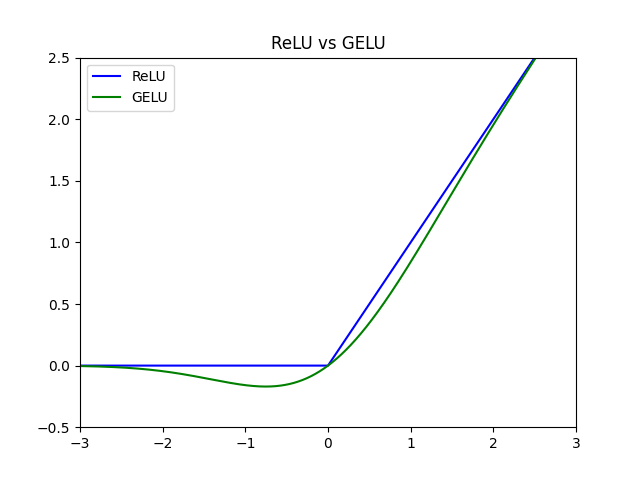
\includegraphics[width=0.9\textwidth]{figures/ml_theory/relu_gelu.png}
		\caption{ReLU and GELU functions}
		\label{fig:relu_gelu}
	\end{subfigure}
	\begin{subfigure}{.5\textwidth}
		\centering
		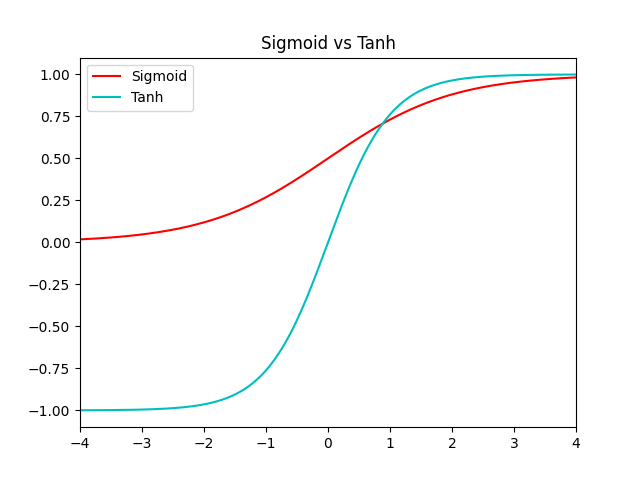
\includegraphics[width=0.9\textwidth]{figures/ml_theory/sigmoid_tanh.png}
		\caption{Sigmoid and Tanh functions}
		\label{fig:sigmoid_tanh}
	\end{subfigure}
	\caption{Activation Functions}
	\label{fig:activation_functions}
\end{figure}

\textbf{ReLU}, defined by
\begin{equation}
\label{eqn:relu_fcn}
\textrm{ReLU}(x) = \max(0, x),
\end{equation}
is a simple function mapping negative values to zero while passing positive values as it is. It is computationally cheap and allows to train deep and complex networks~\cite{glorot_deep_2011}.

\textbf{GELU}, defined by
\begin{equation}
\label{eqn:gelu_fcn}
\textrm{GELU}(x) = x \Phi(x) = \frac{x}{2} \bigg[ 1 + \textrm{erf} \Big( \frac{x}{\sqrt{2}} \Big) \bigg],
\end{equation}
is smoothed version of ReLU function. It is continious but non-convex and has several advantages \cite{hendrycks_gaussian_2020}. ReLU and GELU are visualized in  \figref{fig:relu_gelu}. 

\subsection{Softmax}

Softmax function is generalization upon sigmoid function and used for multinomial classifications. It is smooth type of $\argmax$ operator. Assume that there is a vector $x \in \mathbb{R}^K$. Softmax assigns probability values to each element, summing up to 1. It is defined as,
\begin{equation}
\label{eqn:softmax_fcn}
\text{softmax}(x) = \frac{\exp(x)}{\sum \exp(x)},
\end{equation}
where exponentiation in denominator applied elementwise and denominator is scalar.

\subsection{Layer Normalization}

Layer normalization is a layer to overcome unstablity and divergence during learning~\cite{ba_layer_2016}. 
Given an input $x \in \mathbb{R}^K$, mean and variance statistics are evaluated along the dimensions as  
\begin{equation}
\label{eq:layernorm_statistics}
\begin{split}
\mu = & \frac{1}{K} \sum_{n=1}^{K} x_k \\
\sigma^2 = & \frac{1}{K} \sum_{n=1}^{K} (x_k-\mu)^2
\end{split}.
\end{equation} 
Then, the input is first scaled to have zero mean and unity variance along dimensions. 
The term $\epsilon$ is added to prevent division by zero. 
Optionally, the result is scaled by elementwise multiplication by $\gamma \in \mathbb{R}^K$ and addition by $\beta \in \mathbb{R}^K$ as
\begin{equation}
\label{eqn:layernorm}
\mathrm{LN}(x) = \frac{x-\mu}{\sigma+\epsilon} * \gamma + \beta,
\end{equation}
where $\gamma$ and $\beta$ are learnable parameters. 

\section{Neural Network Types}
\label{sec:nnet_types}

\subsection{Feed Forward Neural Networks (Multilayer Perceptron)}

Structure of perceptron make a way for feed forward neural layers. 
Unlike stated above, a neural layer might output multiple values (say $o \in \mathbb{R}^{1 \times d_o}$) as vector from input (say $x \in \mathbb{R}^{1 \times d_x}$). 
Such a setting forces parameter $W \in \mathbb{R}^{d_x \times d_o} $ to be a matrix. 
Moreover, activation function is not necessarily step function. 
It can be any nonlinear function like sigmoid, tanh, ReLU etc. 
Feed Forward Neural Networks are the generalization of perceptron to approximate any function $f^*$. 
Neural layers are stacked to construct deep feed forward neural network. 
It defines a nonlinear mapping $y=f(x;\theta)$ between input $x$ and output $y$, parametrized by $\theta$ which is set of all learnable parameters like weights, bias and other possible values.

Assuming input signal is $x \in \mathbb{R}^{1 \times d_x}$ (output of previous layer), 
activation value of the layer ($h \in \mathbb{R}^{d_x \times d_h}$) is evaluated as by linear transformation followed by nonlinear activation, 
\begin{equation}
\label{eqn:mlpact}
h = f (x W + b),
\end{equation}
where activation $f$ is applied elementwise.

\subsection{Residual Feed Forward Neural Networks}

As Feed Forward Networks becomes deeper, optimizing weights gets difficult. 
Therefore, people come with the idea of residual connections~\cite{he_deep_2015}. 
For a fixed number of stacked layers (usually 2), input and output of the stack is summed up for next calculations. 
Replacing feed forward layers with other types yield different kind of residual network. 
The difference is demonstrated in \figref{fig:rffnn_ffnn}. 

\begin{figure}
	\centering
	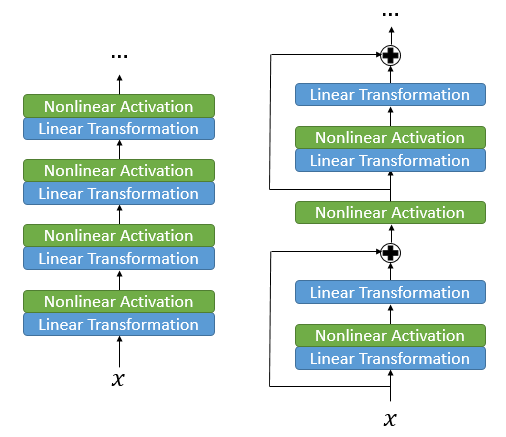
\includegraphics[width=0.5\textwidth]{figures/ml_theory/rffnn_ffnn.png}
	\caption{Deep Feed Forward (left) and Deep Residual Feed Forward Network (right)}
	\label{fig:rffnn_ffnn}
\end{figure}

\subsection{Recurrent Neural Networks}

Recurrent Neural Networks (RNNs) \cite{rumelhart_learning_1986} are type of neural network to process sequential data. 
It is specialized for data having sequential topology. 
It is commonly used for sequence based applications. 

In FFNN layer, output only depends on its input, while Recurrent Layer output is dependent on both input at time $t$ and its output in previous time step $t-1$. 

RNN can be thought as multiple copies of same network which passes message to its successor through time. 
A RNN layer is similar to FFNN layer as in \eqref{eqn:mlpact}, 
except input is concatenation of output feedback and input itself.

Given input sequence $x \in \mathbb{R}^{T \times d_x}$, ,output sequence $h \in \mathbb{R}^{T \times d_h}$ is evaluated recursively,  
\begin{equation}
\label{eqn:rnnact}
h_t = f (h_{t-1} \tilde{W} + x_t W + b)
\end{equation}
where nonlinear activation $f$ \ref{eqn:mlpact} applied element-wise again. Initial output $h_0$ can be either parametrized or assigned as zeros vector. A comparison between FFNN and RNN layer is visualized in \figref{fig:rnn_vs_ffnn}

\begin{figure}
	\centering
	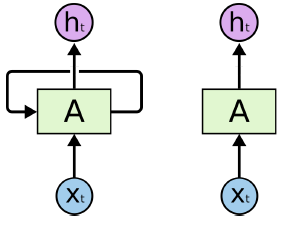
\includegraphics[width=0.5\textwidth]{figures/ml_theory/rnn_vs_ffnn_layer.png}
	\caption{Recurrent Layer (left) and Feed Forward Layer (right) illustration.}
	\label{fig:rnn_vs_ffnn}
\end{figure}

\subsubsection{Long Short Term Memory}

Conventional RNNs have problem with vanishing/exploding gradient problem \cite{olah_understanding_2015}. 
As the sequence gets longer, effect of initial inputs in sequence decreases. 
This causes long term dependence problem. 
If information from initial inputs required, gradients either vanish or explode. 
In order to overcome this problem another architecture is developed called Long Short Term Memory (LSTM)~\cite{hochreiter_long_1997}. 

LSTM is a special type of RNN. 
It is explicitly designed to allow learning long-term dependencies. 
A single LSTM cell has 4 neural layer while vanilla RNN layer has only one neural layer. 
In addition to hidden state $h_t$, there is another state called cell state $C_t$. 
Information flow is controlled by 3 gates. 

\begin{figure}
	\centering
	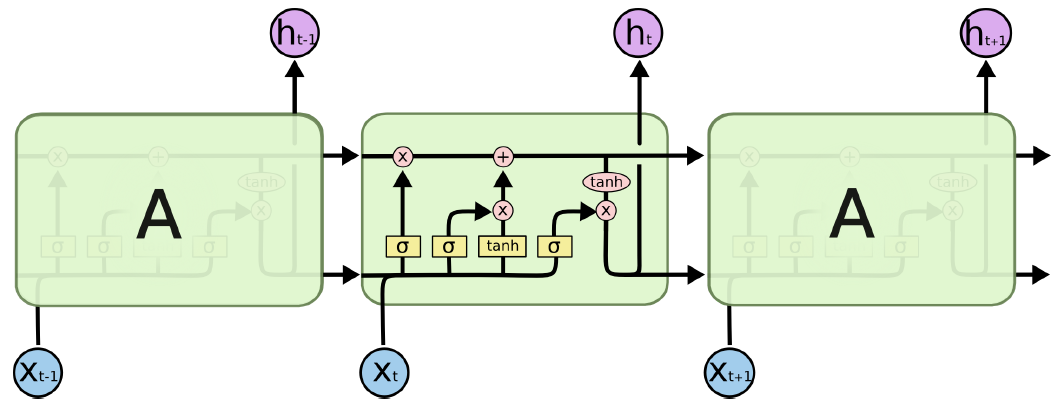
\includegraphics[width=0.98\textwidth]{figures/ml_theory/lstm/lstm_module.png}
	\caption{LSTM Cell}
	\label{fig:lstm_cell}
\end{figure}

\textbf{Forget Gate} controls past memory. 
According to input, past memory is either kept or forgotten. 
Sigmoid function ($\sigma$) is used as activation function, applied elementwise. Mathematically, 
\begin{equation}
\label{eqn:lstm_forget}
f_t = \sigma( [h_{t-1}; x_t] W_f + b_f).
\end{equation}

Hyperbolic tangent layer creates new candidate of cell state from input, 
\begin{equation}
\label{eqn:lstm_cellstcand}
\hat{C}_t = \tanh( [h_{t-1}; x_t] W_C + b_C).
\end{equation}

\textbf{Input Gate} controls contribution from input to cell state (memory), 
\begin{equation}
\label{eqn:lstm_inp}
i_t = \sigma( [h_{t-1}; x_t] W_i + b_{i}).
\end{equation}
Once what are to be forgotten and added decided, cell state is updated as
\begin{equation}
\label{eqn:lstm_cellstupt}
C_t = f_t \odot C_{t-1} + i_t \odot \hat{C}_t.
\end{equation}
using input gate and forget gate outputs.

\textbf{Output Gate} controls which part of new cell state to be output as
\begin{equation}
\label{eqn:lstm_out}
o_t = \sigma( [h_{t-1}; x_t] W_o + b_o).
\end{equation}

Lastly, cell state is filtered by tanh to push values to be in $(-1,1)$ before evaluating hidden state $h_t$ using output gate outputs,
\begin{equation}
h_t = o_t \odot \tanh(C_t).
\end{equation}

\subsection{Attention Mechanism}

As stated earlier, recurrent neural networks are prone to forget long term dependencies. 
LSTM and other variants are invented to overcome this problem. 
Although they reduced this, they cannot attend specific parts of the input. 
Therefore, people came with the idea of weighted averaging all states through time where weights depends on both input and output. 
Assume that input sequence $x \in \mathbb{R}^{T \times d_X}$ is encoded to $h \in \mathbb{R}^{T \times d_H}$. 
The context vector is calculated using weight vector $\alpha \in \mathbb{R}^{1 \times T}$,
\begin{equation}
\mathrm{Attention}(q, h) = \alpha h. %\sum_{\tau=1}^{T} \alpha_{\tau} h_{\tau}.
\label{eq:attention_generic}
\end{equation}

Calculation of weight vector depends on the task. 
For each time step, a score function is calculated between hidden state $h \in \mathbb{R}^{T \times d_H}$ and query $q$ (which may be many things depending on task). 
Attention score is $\alpha \in \mathbb{R}^{T}$ is calculated using predefined arbitrary function $f$ depending on choice. In general form,  
\begin{equation}
\alpha = f(q, h; \theta_{score}).
\end{equation}

\subsubsection{Transformer}

The Transformer was proposed in Attention is All You Need~ \cite{vaswani_attention_2017} paper. 
Unlike recurrent networks, this architecture is solely builded on attention layers. 

A transformer layer consists of feed-forward and attention layers, which makes the mechanism special. 
Like RNNs, it can be used as both encoder and decoder. 
While encoder layers attend to itself, decoder layers attends both itself and encoded input. 

\textbf{Attention Layer} is a mapping from 3 vectors called query $Q \in \mathbb{R}^{T \times d_k}$, key $K \in \mathbb{R}^{T \times d_k}$ and value $V \in \mathbb{R}^{T \times d_v}$ to output, 
where $T$ is time length, $d_k$ and $d_v$ are embedding dimensions. 
Output is weighted sum of values $V$ while weights are evaluated by compatibility metric of query $Q$ and key $K$. 
In vanilla transformer, compatibility of query and key is evaluated by dot product, normalizing by $\sqrt{d_k}$. 
For a query, dot product with all keys are evaluated, then softmax function is applied to get weights of values. Mathematically, 
\begin{equation}
\mathrm{Attention}(Q, K, V) = \mathrm{softmax}(\frac{Q^{T}. K}{\sqrt{d_k}}) V
\end{equation}
This approach is called Scaled Dot-product Attention. 

Instead of performing single attention, \textbf{Multi-Head Attention} projects keys, queries and values linearly from $d_m$ dimensional vector space to $h$ different spaces using projection matrices. 
Then, attention is done $h$ times, and results are then concatenated and linearly projected to final values of the layer.
Projection matrices are model parameters, $W^Q_i \in \mathbb{R}^{d_m \times d_k}$, $W^K_i \in \mathbb{R}^{d_m \times d_k}$, $W^V_i \in \mathbb{R}^{d_m \times d_v}$ for $i=1,...,h$. 
Also output matrix is used to project multiple values into single one, $W^O \in \mathbb{R}^{h d_v \times d_m}$. Mathematically, 
\begin{equation}
\begin{split}
% It is better to write these as \DeclareMathOp
\mathrm{MHA}(Q,K,V) &=  \text{Concat}(\mathrm{head}_1, \mathrm{head}_2, ... \mathrm{head}_h)W^O \\
\mathrm{head}_i &=  \text{Attention}(QW^Q_i,KW^K_i,VW^V_i)
\end{split}.
\end{equation}
Scaled dot-product attention and Multi-Head attention are demonstrated in \figref{fig:att_and_mha}

\begin{figure}
	\centering
	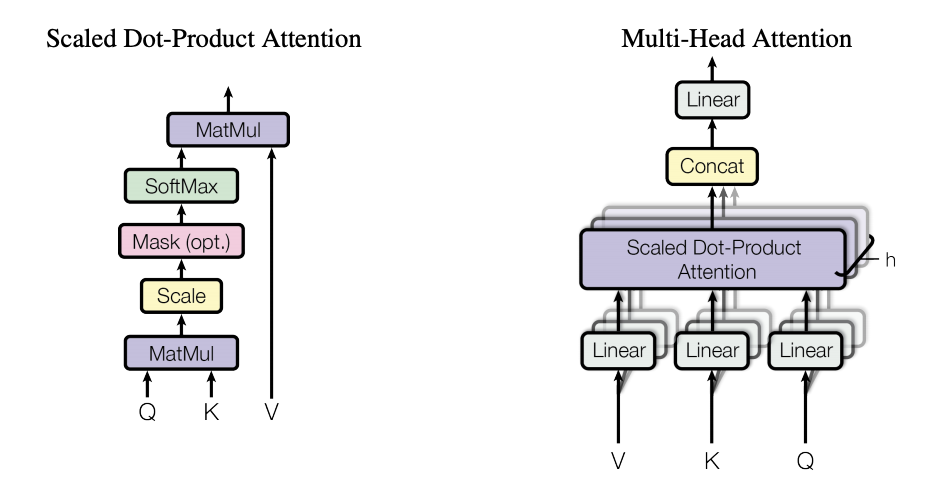
\includegraphics[width=0.98\textwidth]{figures/ml_theory/att.png}
	\caption{Scaled Dot-Product Attention (left) and Multi-Head Attention (right)}
	\label{fig:att_and_mha}
\end{figure}

Both encoder and decoder contains \textbf{Feed Forward Layer}, containing two linear transformations with ReLU activation.
\begin{equation}
\mathrm{FFN}(x) = \text{ReLU}(xW_1+b)W_2+b_2
\end{equation}

\textbf{Encoder Layer} starts with a residual self attention layer. 
Self attention means that query, key and value are the same vectors. 
Then it is followed by feed forward neural layer. 
Both sublayers are employed with resudial connection with layer normalization, 
i.e summation of layer input and output is passed through layer normalization. 
\begin{equation}
\begin{split}
a = & \mathrm{LN}(x + \mathrm{MHA}(x,x,x)) \\
y = & \mathrm{LN}(a + \mathrm{FFN}(att))
\end{split}
\end{equation}

\textbf{Decoder Layer} has also self-attention and feed forward layers similar to encoder layer. 
In addition, there is another attention layer which is over encoder outputs. 
Same as encoder, all sublayers have residual connection with layer normalization. 
Let's call encoded sequence $e \in \mathbb{R}^{T \times d_m}$ and decoded sequence $d \in \mathbb{R}^{T \times d_m}$ (masked). 
Assume that the sequence decoded up to $t$th point in sequence. 
Then, $d_{t+1}$ is calculated as follows. 
\begin{equation}
\begin{split}
a = & \mathrm{LN}(d_{1:t}+\mathrm{MHA}(d_{1:t},d_{1:t},d_{1:t})) \\
s = & \mathrm{LN}(a + \mathrm{MHA}(a,e,e)) \\
d_{t+1} = & \mathrm{LN}(s+ \mathrm{FFN}(s))
\end{split}
\end{equation}

Since there are no recurrent or convolutional architecture in the model, sequential information needs to be embedded. 
For this purpose, \textbf{Positional encoding}s are used. 
They have same dimension with input $x$, so that input embeddings can be added to at the beginning of encoder or decoder stacks. 
For position $p$, $2i$ or $2i+1$th dimension has following values ($i \in \mathbb{N}$), 
\begin{equation}
\begin{split}
\mathrm{PE}_{p,2i} = \sin(pos/10000^{2i/d_m}) \\
\mathrm{PE}_{p,2i+1} = \cos(pos/10000^{2i/d_m})
\end{split},
\end{equation}
as proposed in the original paper. 

\subsubsection{Pre-Layer Normalized Transformer}

Original transformer architecture includes layer normalization operations after attention and feed-forward layers. 
It is unstable since the values of gradients of output layers are high, so Pre-Layer Normalized transformer is proposed by \cite{xiong_layer_2020} by carrying layer normalization operation to in front of attention and feed-forward layers. 
Moreover, Parisotto et al. Xiong et al.~ \cite{parisotto_stabilizing_2019} proposed gated transformer which also includes layer normalizations before attention and feedforward layer. 
They also stated that although gated architecture improves many RL tasks drastically, non-gated pre-layer normalized transformer are good enough. 

In pre-layer normalized transformer, encoder equations are as follows,
\begin{equation}
\begin{split}
a = & x+ \mathrm{MHA}(\mathrm{LN}(x),\mathrm{LN}(x),\mathrm{LN}(x)) \\
y = & a + \mathrm{FFN}(\mathrm{LN}(a))
\end{split}.
\end{equation}
The difference between post-layer and pre-layer transformer encoders are visualized in \figref{fig:post_pre_trsf}

\begin{figure}
	\centering
	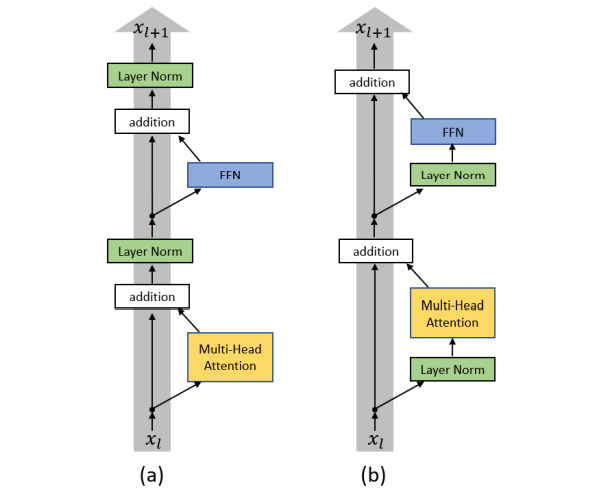
\includegraphics[width=0.7\textwidth]{figures/ml_theory/post_pre_trsf.png}
	\caption{(a) Post-LN Transformer layer, (b) Pre-LN Transformer
		layer.}
	\label{fig:post_pre_trsf}
\end{figure}

%Decoder equations are as follows.
%\begin{equation}
%\begin{split}
%att = & %d_{1:t}+\mathrm{MHA}(\mathrm{LN}(d_{1:t}),\mathrm{LN}(d_{1:t}),\mathrm%{LN}(d_{1:t})) \\
%dec = & att+ \mathrm{MHA}(\mathrm{LN}(att),\mathrm{LN}(att),\mathrm{LN}(att)) \\
%d_{t+1} = & dec+ \mathrm{FFN}(\mathrm{LN}(dec))
%\end{split}
%\end{equation}


\chapter{INTRODUCTION}
\label{chap:intro}

Artificial intelligence is the ability of a computer program 
or a machine to think and learn like natural intelligence 
performed by humans and animals. 
One way is to create an intellgent agent is using pattern detection  methods on data and use it to make predictions on unseen data. 
This approach is called Machine Learning. 

Humans and animals exhibit several different behaviours in terms of 
interaction with environment, such as utterance and movement. 
Their behavior is based on past experience, the situation they are in  and their objective. 
Like humans and animals, an intelligent agent is expected to take 
action according to its perception based some objective. 
A major challenge to machine learning is creating agents that will 
act more natural and humanlike. 
As a subfield of Machine Learning, Reinforcement Learning allows an 
agent to learn how to control (or act) itself in different situations by interaction with environment. 
In RL, environment is modeled to give reward or punishment to agent 
according to environmental state and agent actions, and agent focuses
on learning to predict what actions will lead to highest reward 
(or lowest punishment, based on its objective) in the future using past experience. 

Traditional RL algorithms need feature engineering from observation. 
For complex problems, the way to extract features is ambiguous or 
observations are not enough to create a good model. 
As a newer  technique, deep neural networks allows to extract 
high level features from data with large state-space 
(pixelwise visual, many kinematic sensors etc.) and missing  observations. 
Along with recent developments in DNNs, Deep Reinforcement Learning 
allows an agent to interact with environment in more complex way. 
DRL is based on neural networks which are function approximators. 
The problem with DRL is selection of a correct neural network, 
but there is still no analytical method to design a neural network for a particular task. 
Therefore, neural design is commonly based on trial-error. 

Since its discovery, robots have been crucial devices for the human race, whether smart or not. 
Intelligent humanoid and animaloid robots have been in 
continuous development since early 1980s. 
This type of robots has legs unlike driving robots. 
Since most of world terrain is unpaved, this type of robots are good alternative to driving robots. 
Locomotion is major task for such robots. Stable bipedal (2 legged)  walking 
is one of the most challenging problem among the control problems. 
It is hard to create accurate model due to high order of dynamics,  friction and discontinuities. 
Even so, design of walking controller using traditional methods is difficult due to same reasons. 
Therefore, for bipedal walking, DRL approach is an easier choice if a simulation environment is available. 

In this thesis, Bipedal Locomotion Deep Reinforcement Learning (DRL) by is investigated through \textit{BipedalWalker-Hardcore-v3} \cite{noauthor_bipedalwalkerhardcore-v2_2021} environment of open source GYM library \cite{brockman_openai_2016}. Different neural architectures are used and results are compared. 

\section{Proposed Neural Networks}
\label{sec:proposed_networks}

For all networks, varing backbones used to encode state information from observations for both actor and critic networks. 
In critic network, actions are concatenated by state information coming from backbones. 
Then, this concatenated vector is passed through feed forward layer with GELU activation then a linear layer with single output. 
Before feeding observations to backbone, they are passed through a layer with layer normalization with tanh activation to 96 dimensional output. 
In actor network, backbone is followed by a single layer with tanh activation for action estimation. 
As backbones, following networks are proposed. 
Again, observations are passed through a layer with layer normalization with tanh activation to 96 dimensional output before feeding to backbone. 
Critic and Actor networks are illustrated in \figref{fig:nets} 

\begin{figure}
	\begin{subfigure}{.5\textwidth}
		\centering
		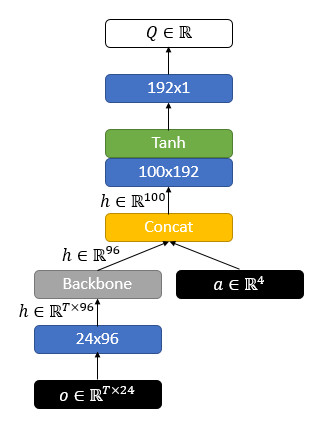
\includegraphics[width=0.97\linewidth]{figures/nets/critic.png}
		\caption{Critic Architecture}
		\label{fig:critic_net}
	\end{subfigure}
	\begin{subfigure}{.5\textwidth}
		\centering
		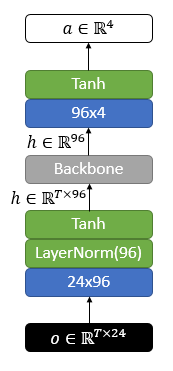
\includegraphics[width=0.55\linewidth]{figures/nets/actor.png}
		\caption{Actor Architecture}
		\label{fig:actor_net}
	\end{subfigure}
	\caption{Neural Architecture Design}
	\label{fig:nets}
\end{figure}

\subsection{Residual Feed Forward Network}

Incoming vector is passed through 2 layers with 192 dimensional hidden size and 96 dimensional output, where there is GELU activation between 2 layers. 
This output is summed with initial vector and this is lastly passed through layer normalization. 

\subsection{Long Short Term Memory}

Sequence of incoming vectors is passed though single layer vanilla LSTM layer with 96 dimensional hidden state. 
Output at last time step is outputted. 

\subsection{Transformer (Pre-layer Normalized)}

Sequence of incoming vectors is passed through single layer pre-layer normalized transformer with 192 dimensional feed forward layer with GELU activation. 
The output is lastly passed through layer normalization. 
During multi-head attention, only the last state is fed as query so that attentions are calculated for only last state. 


\section{RL Method and Hyperparameters}
\label{sec:rlmethod}

TD3 and SAC is used as RL algorithm. 
Hyperparameters are selected by grid search and best performing values are used. Adam optimizer is used for optimization. 

In TD3, as exploration noise, Ornstein-Uhlenbeck noise is used, and standart deviation is multiplied  by $0.999$ at the end of each episode. 

All hyperparameters are found after a trial-error process. They  are summarized in \tabref{table:hyperparams_td3} and \tabref{table:hyperparams_sac}. Unlisted ones have default values which PyTorch gives. 

\begin{table}
	\begin{tabular}{|l||*{3}{c|}}\hline
		\backslashbox{Hyperparameter}{Model}
		&\makebox[5em]{RFFNN}&\makebox[5em]{LSTM}&\makebox[5em]{Transformer}\\\hline\hline
		$\eta$ (Learning Rate) & $1.0\times10^{-3}$ & $7.0\times10^{-4}$ & $1.0\times10^{-3}$\\\hline
		$\beta$ (Momentum) & \multicolumn{3}{|c|}{$(0.9, 0.999)$}\\\hline
		$\gamma$ (Discount Factor) & \multicolumn{3}{|c|}{$0.98$} \\\hline
		$N_{replay}$ (Replay Buffer Size) &\multicolumn{3}{|c|}{$500000$} \\\hline
		$N$ (Batch Size) &\multicolumn{3}{|c|}{$128$}\\\hline
		$d$ (Policy Delay) &\multicolumn{3}{|c|}{$2$}\\\hline
		$\sigma$ (Policy smoothing std) &\multicolumn{3}{|c|}{$0.2$}\\\hline
		$\tau$ (Polyak parameter) &\multicolumn{3}{|c|}{$0.005$}\\\hline
		Exploration &\multicolumn{3}{|c|}{$OU(\theta=4.0, \sigma=1.0)$}\\\hline
	\end{tabular}
	\caption{Hyperparmeters and Exploration of Learning Processes for TD3}
	\label{table:hyperparams_td3}
\end{table}
\noindent

\begin{table}
	\begin{tabular}{|l||*{3}{c|}}\hline
		\backslashbox{Hyperparameter}{Model}
		&\makebox[5em]{RFFNN}&\makebox[5em]{LSTM}&\makebox[5em]{Transformer}\\\hline\hline
		$\eta$ (Learning Rate) & $1.0\times10^{-3}$ & $1.0\times10^{-3}$ & $1.0\times10^{-3}$\\\hline
		$\beta$ (Momentum) & \multicolumn{3}{|c|}{$(0.9, 0.999)$}\\\hline
		$\gamma$ (Discount Factor) & \multicolumn{3}{|c|}{$0.98$} \\\hline
		$N_{replay}$ (Replay Buffer Size) &\multicolumn{3}{|c|}{$500000$} \\\hline
		$N$ (Batch Size) &\multicolumn{3}{|c|}{$128$}\\\hline
		$\tau$ (Polyak parameter) &\multicolumn{3}{|c|}{$0.005$}\\\hline
		$\alpha$ (Entropy Temperature) &\multicolumn{3}{|c|}{$0.01$}\\\hline
	\end{tabular}
	\caption{Hyperparmeters and Exploration of Learning Processes for SAC}
	\label{table:hyperparams_sac}
\end{table}
\noindent

\section{Results}

For each episode, episode scores are calculated by summing up rewards of each time step. 
In \figref{fig:td3_scatter_ep_rewards} and \figref{fig:sac_scatter_ep_rewards}, a scatter plot is visualized for each model's episode scores. 
In \figref{fig:td3_std_ep_rewards} and \figref{fig:sac_std_ep_rewards}, moving average and standard deviation is visualized for each model's episode scores. 

\begin{figure}[!ht]
	\centering
	\begin{subfigure}{.49\textwidth}
		\centering
		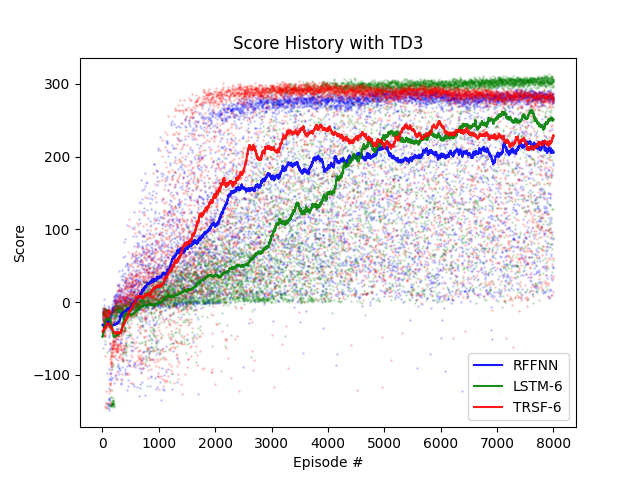
\includegraphics[width=0.99\textwidth]{figures/bipedal/SCT_TD3_RFFNN_LSTM-6_TRSF-6.png}
		\caption{TD3}
		\label{fig:td3_scatter_ep_rewards}
	\end{subfigure}
	\begin{subfigure}{.49\textwidth}
		\centering
		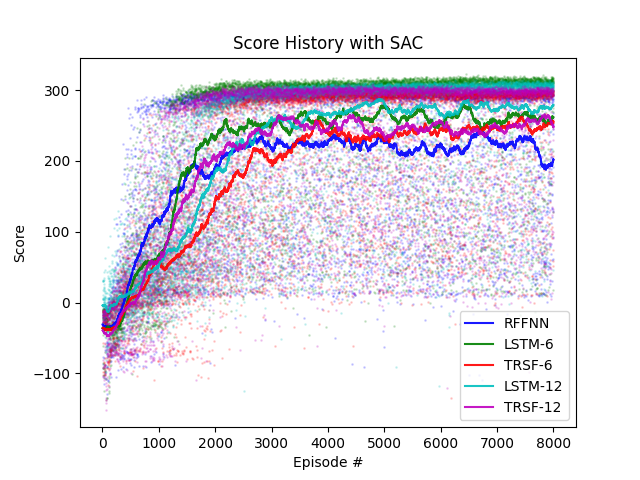
\includegraphics[width=0.95\textwidth]{figures/bipedal/SCT_SAC_RFFNN_LSTM-6_TRSF-6_LSTM-12_TRSF-12.png}
		\caption{SAC}
		\label{fig:sac_scatter_ep_rewards}
	\end{subfigure}
	\caption{Scatter Plot with Moving Average for Episode Scores}
\end{figure}

\begin{figure}[!ht]
	\centering
	\begin{subfigure}{.49\textwidth}
		\centering
		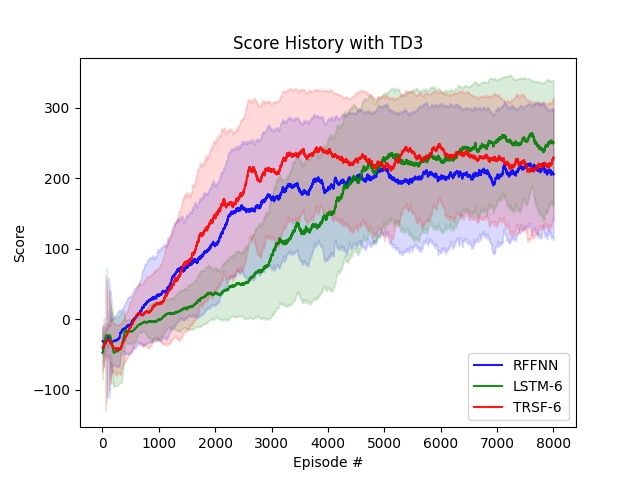
\includegraphics[width=0.99\textwidth]{figures/bipedal/STD_TD3_RFFNN_LSTM-6_TRSF-6.png}
		\caption{TD3}
		\label{fig:td3_std_ep_rewards}
	\end{subfigure}
	\begin{subfigure}{.49\textwidth}
		\centering
		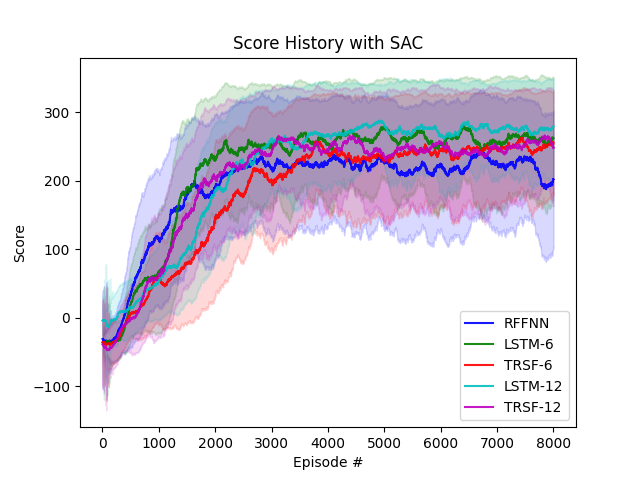
\includegraphics[width=0.95\textwidth]{figures/bipedal/STD_SAC_RFFNN_LSTM-6_TRSF-6_LSTM-12_TRSF-12.png}
		\caption{SAC}
		\label{fig:sac_std_ep_rewards}
	\end{subfigure}
	\caption{Moving Average and Standard Deviation for Episode Scores}
\end{figure}

Officially, 300 points in average required in random 100 simulations to say the environment is solved.
Therefore, none of our approaches solved.
However, they partially solved problems by exceeding 200 point limit, while some simulations yield around 280 points with all neural networks in TD3 and 300 points are reached with SAC. 

RFFNN seems to be enough for solving the problem, although there exist partial observability in the environment. 
That model reaches around 220 points in average with TD3 and 225 points with SAC. In addition, learning was unstable. 

The robot was able to walk by LSTM model but yield worse results and cannot exceed 120 points in average with both TD3 and SAC. 

Transformer model yield best results by reaching 230 points with TD3 and exceeds 250 points with SAC. 

As Transformer and RFFNN are relatively succesfull, their behavior is visualized in \figref{fig:rffnn_simulation} and \figref{fig:trsf_simulation} for TD3 model. 
The main behavioral difference is when the agent faces a big hurdle. 
First model passes it by jumping while other does by taking a very big step, shown in \figref{fig:anim_rffnn_hurdle} and \figref{fig:anim_trsf_hurdle}.

In SAC results, RFFNN and Transformer agents do not exhibit a noteworthy difference.

Also, SAC model performes better than TD3 in general. 
Agent cannot exceed 280 points in any simulation with TD3 (\figref{fig:td3_scatter_ep_rewards}) but it exceeds 300 points with SAC (\figref{fig:sac_scatter_ep_rewards}). Also, as seen from the moving average points, SAC agents are superior (\figref{fig:td3_std_ep_rewards},\figref{fig:sac_std_ep_rewards}).

\begin{figure}[!ht]
	\centering
	\begin{subfigure}{.95\textwidth}
		\centering
		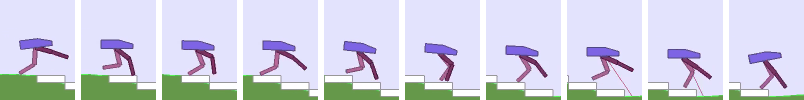
\includegraphics[width=0.95\textwidth]{figures/bipedal/anim/ff-stairs.png}
		\caption{Stairs}
		\label{fig:anim_rffnn_stairs}
	\end{subfigure}
	\begin{subfigure}{.95\textwidth}
		\centering
		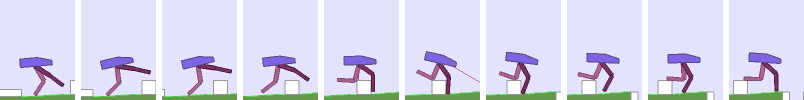
\includegraphics[width=0.95\textwidth]{figures/bipedal/anim/ff-hurdle.png}
		\caption{Hurdle}
		\label{fig:anim_rffnn_hurdle}
	\end{subfigure}
	\begin{subfigure}{.95\textwidth}
		\centering
		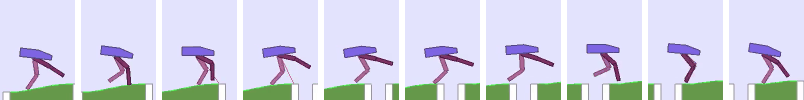
\includegraphics[width=0.95\textwidth]{figures/bipedal/anim/ff-pitfall.png}
		\caption{Pitfall}
		\label{fig:anim_rffnn_pitfall}
	\end{subfigure}
	\caption{Walking Simulation of RFFNN model at best version with SAC}
	\label{fig:rffnn_simulation}
\end{figure}

\begin{figure}[!ht]
	\centering
	\begin{subfigure}{.95\textwidth}
		\centering
		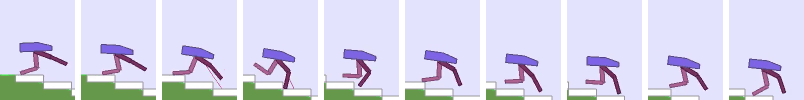
\includegraphics[width=0.95\textwidth]{figures/bipedal/anim/lstm-12-stairs.png}
		\caption{Stairs}
		\label{fig:anim_lstm_stairs}
	\end{subfigure}
	\begin{subfigure}{.95\textwidth}
		\centering
		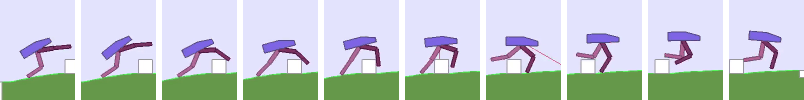
\includegraphics[width=0.95\textwidth]{figures/bipedal/anim/lstm-12-hurdle.png}
		\caption{Hurdle}
		\label{fig:anim_lstm_hurdle}
	\end{subfigure}
	\begin{subfigure}{.95\textwidth}
		\centering
		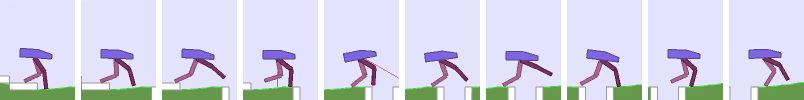
\includegraphics[width=0.95\textwidth]{figures/bipedal/anim/lstm-12-pitfall.png}
		\caption{Pitfall}
		\label{fig:anim_lstm_pitfall}
	\end{subfigure}
	\caption{Walking Simulation of LSTM-12 model at best version with SAC}
	\label{fig:lstm_simulation}
\end{figure}

\begin{figure}[!ht]
	\centering
	\begin{subfigure}{.95\textwidth}
		\centering
		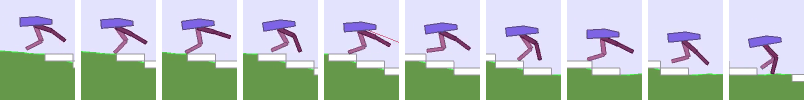
\includegraphics[width=0.95\textwidth]{figures/bipedal/anim/trsf-12-stairs.png}
		\caption{Stairs}
		\label{fig:anim_trsf_stairs}
	\end{subfigure}
	\begin{subfigure}{.95\textwidth}
		\centering
		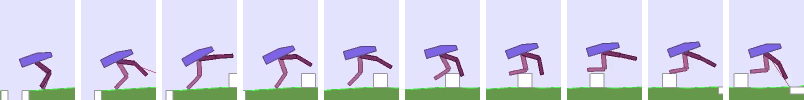
\includegraphics[width=0.95\textwidth]{figures/bipedal/anim/trsf-12-hurdle.png}
		\caption{Hurdle}
		\label{fig:anim_trsf_hurdle}
	\end{subfigure}
	\begin{subfigure}{.95\textwidth}
		\centering
		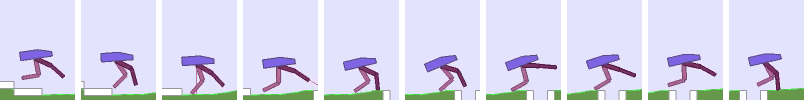
\includegraphics[width=0.95\textwidth]{figures/bipedal/anim/trsf-12-pitfall.png}
		\caption{Pitfall}
		\label{fig:anim_trsf_pitfall}
	\end{subfigure}
	\caption{Walking Simulation of Transformer-12 model at best version with SAC}
	\label{fig:trsf_simulation}
\end{figure}

\section{Discussion}
We believe that these results are not enough to conclude on a superior neural network for all RL problems, because there are other factors such as DRL algorithm, number of episodes, network size etc. 
However, networks are designed to have similar sizes and good model requires to converge in less episodes. 
As a result, LSTM is superior to Transformer for our environment. 
In addition, it is possible to conclude that Transformers can be an option for partially observed RL problems, thanks to incorprating observation history. 
Note that this is valid where layer normalization is applied before multihead attention and feed-forward layers \cite{xiong_layer_2020} as opposed to vanilla transformer proposed in \cite{vaswani_attention_2017}. 

Another result is that incorprating past observations did improve performance significantly since environment is partially observable.
Especially increasing history length keeps increasing performance for both LSTM and Transformer models. 

The environment is a difficult one. 
There are really few available models which gets close to a solution~~\cite{noauthor_gymleaderboard_2021}. 
Apart from neural networks, there are other factors affecting performance such as RL algorithm, rewarding, exploration etc. 
In this work, all of them are adjusted such that the environment becomes solvable. 
Time frequency is reduced for sample efficiency and speed. 
Also, the agent is not informed for the terminal state when it reaches time limit. 
Lastly, punishment of falling reduced, so the agent is allowed to learn by mistakes. 
We believe that those modifications are also source of our high performance. 

As RL algorithm, TD3 is selected first, since it is a good choice for continuous RL. 
Ornstein-Uhlenbeck noise is used for better exploration since it has momentum, and its variance is reduced by time to make agent learn small actions well in later episodes. 
However, we cannot feed 12 observation history to sequential models since TD3 failed to learn in that case.
In addition, SAC is used for learning along with TD3. 
Results are better compared to those of TD3. 
SAC policy maximizes randomness (entropy) if agent cannot get sufficient reward and this allows the agent to decide where/when to explore more or less. 
This way, SAC handles the sparse rewards from the environment better than TD3. 

\chapter{CONCLUSION AND FUTURE WORK}
\label{chap:conclusion_future_work}

\section{Conclusion}
\label{sec:conclusion}
In this thesis, bipedal robot walking is investigated by deep  reinforcement learning due to complex dynamics. 
For real world robot control by RL, simulation is an important step. 
Usually, models are pretrained in simulation environment before learning in reality due to safety and exploration reasons. 

TD3 algorthim is used since it is robust and well suited for continious control. 
Also, environment is slightly modified by reward shaping, halving simulation frequency, cancelling terminal state information at time limit so that learning becomes easier.  
As stated in previous chapters, most of the real world environments are partially observable. 
In BipedalWalker-Hardcore, the environment is also partially observable since agent cannot observe behind of it lacks of acceleration sensors which is better to have for controlling mechanical systems. 
Therefore, we used Long Short Term Memory and Transformer Neural Networks to capture more information from past observations compared to Residual Feed Forward Neural Network (RFFNN) using single instant observation as input. 

RFFNN model performed well thanks to carefully selected hyperparameters and modifications on the environment. 
Since there is no major differences between sequential models (Transformer), the problem is mainly about rewards and exploration, not partial observability. 

Although LSTM is used commonly for partially observed problems, results are worst compared to other two models, but keeps learning slowly. 
Without knowing exact reason, it is probably its functional properties. 

Transformer model worked with best performance among all models. 
It is surprising because it is not succesfully used in RL problems in general. 
In natural language processing, this type of attention models completely replaced recurrent models, and our results seems promising for this in RL domain. 


\section{Future Work}
\label{sec:future_work}

There might be a few possible ways to improve this work. 
First of all, longer observation history can be used to handle partial observability for LSTM and Transformer models. 
However, this makes learning slower and difficult and requires more stable RL algorithms and fine tuning on hyperparameters. 
Secondly, different exploration strategies might be followed. 
Especially parameter space exploration \cite{plappert_parameter_2018} may perform better since it works better for environments with sparse reward like our environment. 
Lastly, advanced neural networks and RL algorithms (specificly designed for environment) may be designed by incorprating domain knowledge. 



%
% References in Bibtex format goes into below indicated file with .bib extension
\bibliography{myBiblio} % filename: myBiblio.bib
% You can use full name of authors, 
% however most likely some of the Bibtex entries you will find, 
% will use abbreviated first names.
% If you don't want to correct each of them by hand, 
% you can use abbreviated style for all of the references
%\bibliographystyle{abbrv}
% However, IAM suggests to use
\bibliographystyle{iamBiblioStyle} % better than to use {plain or abbrv}
%%% APPENDIXES
\appendix
%
% input your appendix
% If you are not using minted style, then comment the first appendix below
% otherwise uncomment.
%uncomment%  \chapter{Proof of Some Theorem}
\label{app:mintedCodes}

This is appendix text.

\definecolor{myBgColour}{rgb}{0.99,0.99,0.99} % almost white

\setminted[python]{frame=single,
framesep=2mm,
baselinestretch=1.1,
bgcolor=myBgColour,
fontsize=\footnotesize,
linenos, autogobble,
python3=true}

\setminted[matlab]{frame=single,
framesep=2mm,
baselinestretch=1.1,
bgcolor=myBgColour,
fontsize=\footnotesize,
linenos, autogobble,
python3=true}

%\captionsetup[Listing]{format=plain,font={small},labelfont={bf}, aboveskip=-5px}
%\renewcommand{\theListing}{{\arabic{Listing}}}
%\setcounter{Listing}{0}


However, we place a python code here with a listing environment
Listing~\ref{lst:first}.	

\begin{listing}	
\begin{minted}{python}
# Python program to check if the input number is prime or not

num = 407

# take input from the user
# num = int(input("Enter a number: "))

# prime numbers are greater than 1
if num > 1:
   # check for factors
   for i in range(2,num):
       if (num % i) == 0:
           print(num,"is not a prime number")
           print(i,"times",num//i,"is",num)
           break
   else:
       print(num,"is a prime number")
       
# if input number is less than
# or equal to 1, it is not prime
else:
   print(num,"is not a prime number")
\end{minted}
\caption{This is the caption of this Listing environment\label{lst:first}}
\end{listing}

Also we wish to insert a MATLAB code, too.

\definecolor{myBackgroundColour}{rgb}{0.9,0.9,0.9} % almost gray
\begin{minted}[
frame=lines,
framesep=2mm,
baselinestretch=1.2,
bgcolor=myBackgroundColour,
fontsize=\footnotesize,
linenos
]{matlab}
function result = myprime(n)
% MATLAB program to check if the input number is prime or not

%% initially set output flag to true
 result = true;
%% iterate over all positive integers 2,3,...,n-1
%% if n is not divisible by any of these factors....it is prime
 if (n == 1)
     result = 'false';
 elseif (n == 2)
     result = 'true';
 else 
    for i=2:n-1,
        if (mod(n,i)==0)
           result = 'false';
        end
    end
 end
%% return "true" or "false" instead of 1 or 0  
 if (result)
    result = 'true';
 else
    result = 'false';
 end
\end{minted}


Furthermore, here are two files (myPythonCode.py and myMatlabCode.m) included.

\inputminted[
frame=single,
framesep=2mm,
baselinestretch=1.2,
bgcolor=myBackgroundColour,
fontsize=\footnotesize,
linenos
]{python}{myPythonCode.py}

\definecolor{myRed}{rgb}{0.95,0.1,0.1}

\begin{listing}
\inputminted[frame=single, linenos, bgcolor=myRed]{matlab}{myMatlabCode.m}
\caption{Here is the caption again}
\end{listing} % includes minted package examples!
%\chapter{Proof of Some Theorem}
\label{app:somethms}

This is appendix text.

\begin{listing}
  %\VerbListingBoxed{myMatlabCode.m}
  \VerbatimInput{myMatlabCode.m}
	%\inputminted{matlab}{myMatlabCode.m} % only if minted is used!
  %\VerbListing{myMatlabCode.m}
\caption{The \texttt{lintest} function in a floating ``listing'' environment.}
\label{mfile:linetest-3}
\end{listing}


%
%
% If you are a Ph.D. Student you need to insert a CV at the end of you thesis
% Check vita.tex for a simple CV template in Latex
%\curriculumvitae
\label{chapter:vita}

\section*{\uppercase{Personal Information}}

\textbf{Surname, Name: } Surname, Name\\
\textbf{Nationality:} Turkish (TC) \\
\textbf{Date and Place of Birth:} dd.mm.yyyy, City\\
\textbf{Marital Status:} Single \\
\textbf{Phone:} 0 312 0000000 \\
\textbf{Fax:} 0 312 0000000 \\

\section*{\uppercase{Education}}

\begin{tabular}{lll}
\textbf{Degree} & \textbf{Institution} & \textbf{Year of Graduation} \\
M.S. & M.S. Institute & M.S. Year \\
B.S. & B.S. Institute & B.S. Year \\
High School & High School Name & High School Graduating Year
\end{tabular}

\section*{\uppercase{Professional Experience}}

\begin{tabular}{lll}
\textbf{Year} & \textbf{Place} & \textbf{Enrollment} \\
Duration 1 & Institute/Company 1 & Role/Position/Experience 1 \\
Duration 2 & Institute/Company 2 & Role/Position/Experience 2 
\end{tabular}

\section*{\uppercase{Publications}}
\subsection*{International Conference Publications}
Your publications goes here. Do not try to use Bibtex, since Bibtex builds a single bibliography
database for the document.

\end{document}
